\chapter{Wing Box model} \label{chap:Model}

\section{Introduction} \label{sec:intro_Model}

% Introduction to the chapter

\section{Concept} \label{sec:concept_Model}

% Explanation of the concept
% -> Bending-twist coupling
% -> Shiftable shear centre location
% -> A web with variable-stiffness capability

% Figure: Fig. 1 Raither ?, Geometry and system of coordinates.
% Figure: Fig. 2 Raither ?, Schematic of the working principle.

% -> Buckling phenomena
% Figure: Schematic representation buckling phenomena

\section{Analytical model} \label{sec::analytical_Model}

%% Analytical apprach description
% An analytical model of the Wing Box will be build.
% Shear centre calculation
% The twist of the beam will be calculated
%
%Figure of analytical model
\begin{figure}[!htpb]
  \centering
  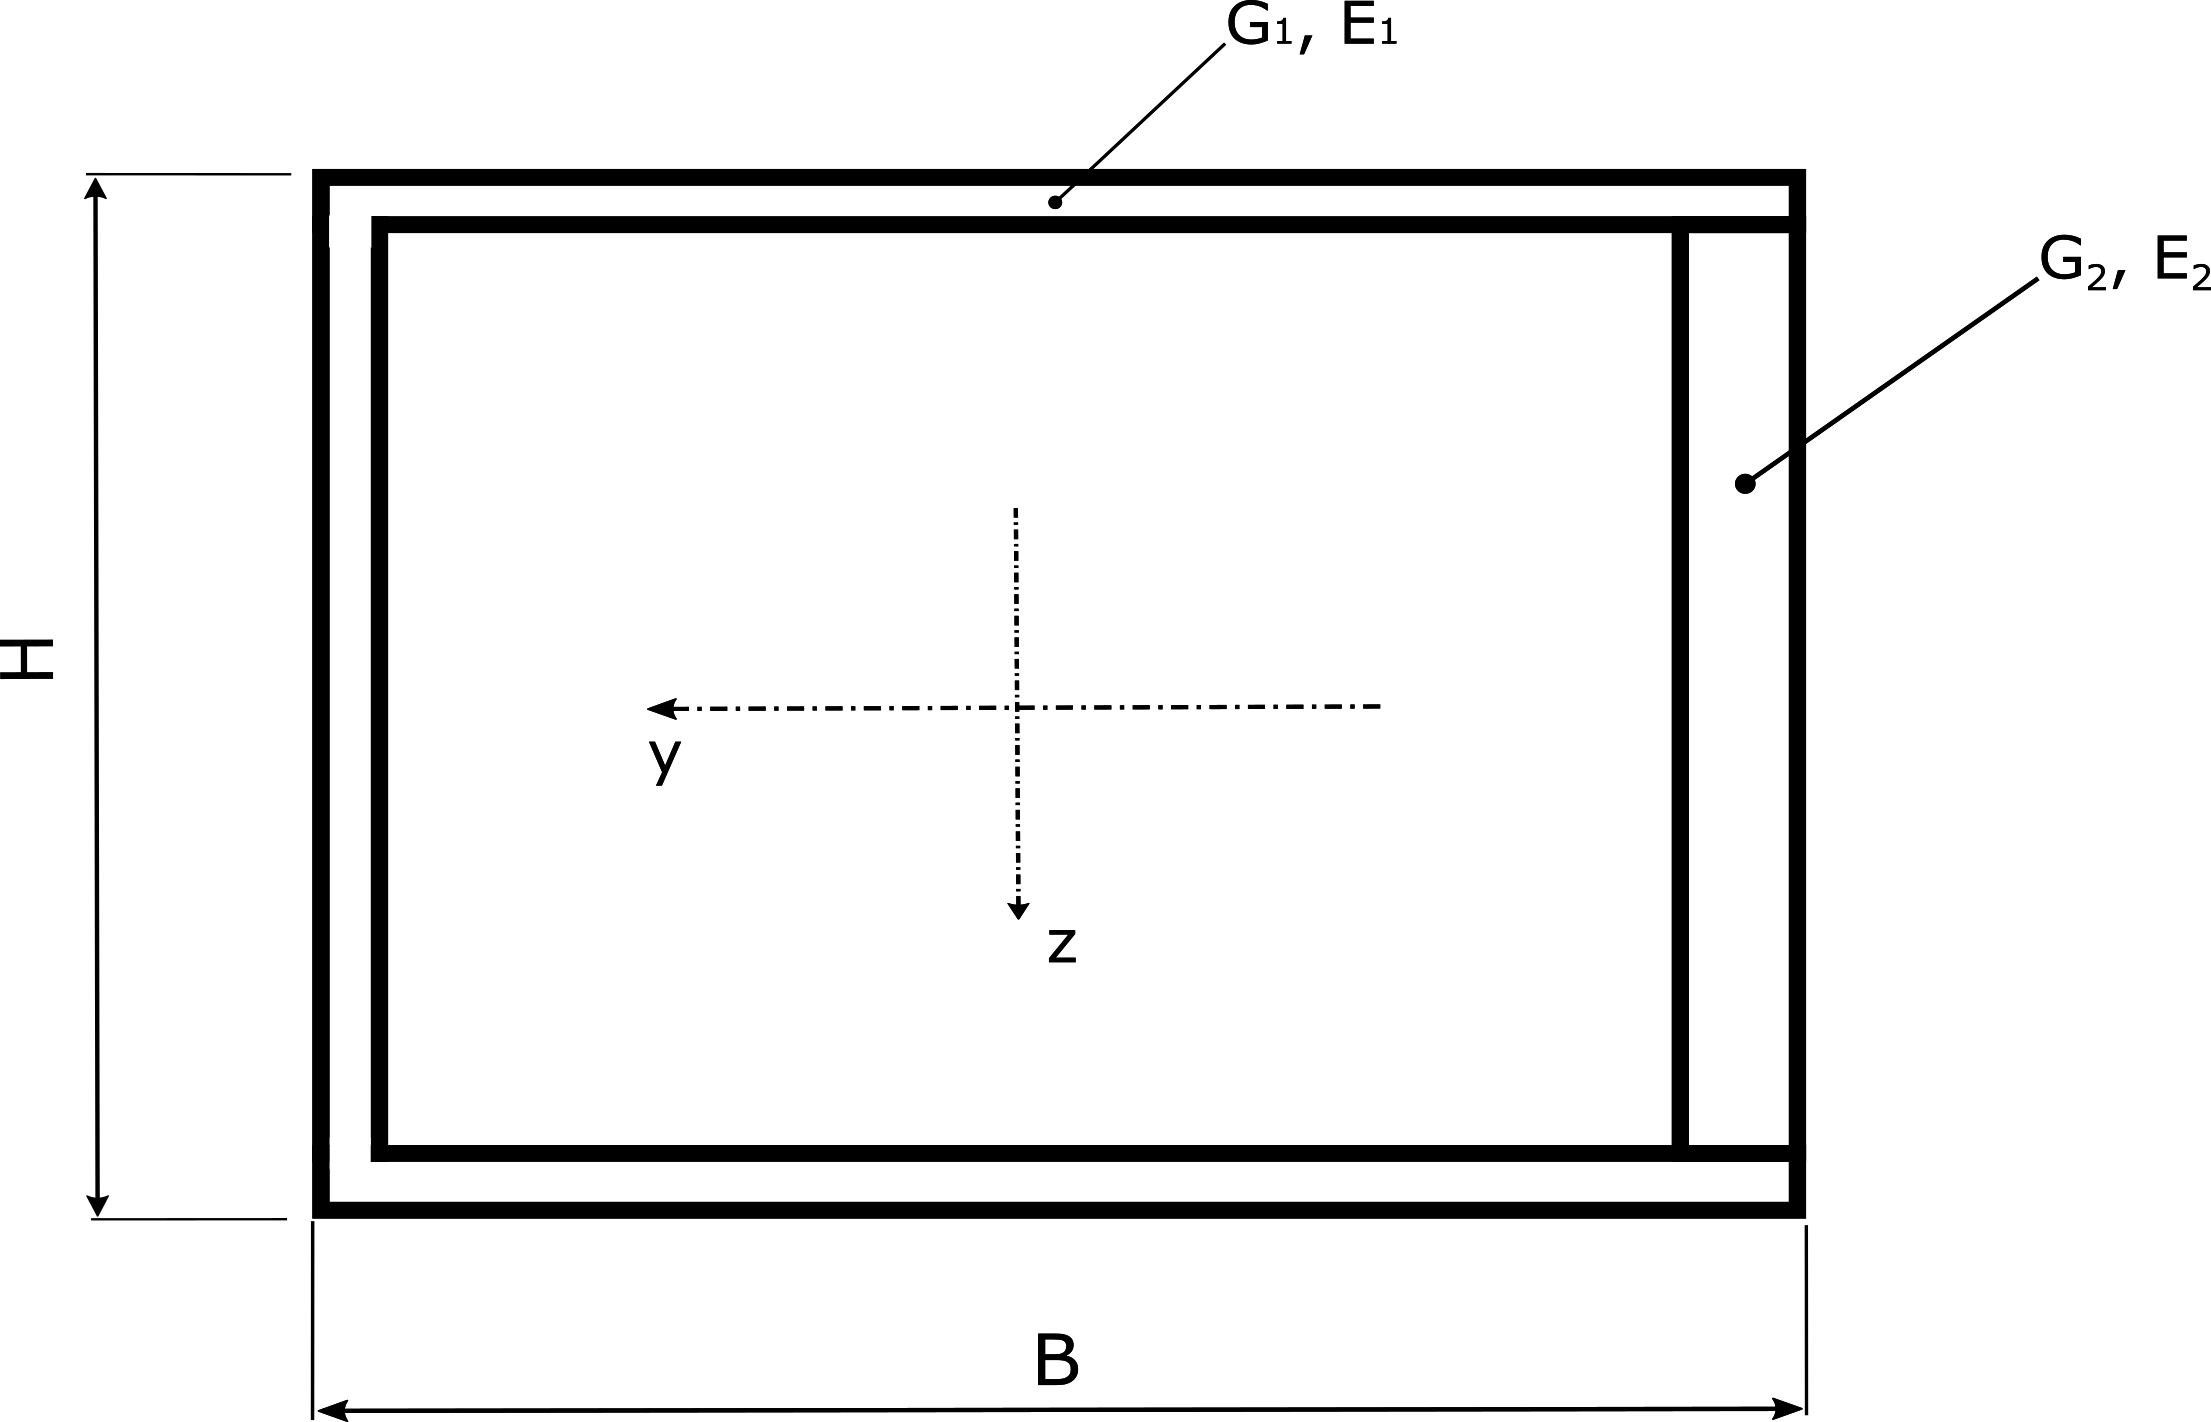
\includegraphics[width=0.8 \textwidth]{model/analyticalBox}
  \caption[Schematic view of the beam closed section]{Schematic view of the beam closed section. The dimensions are given by the width $B$ and the height $H$. For the upper, lower and left elements, the shear modulus and the elastic modulus are given by $G_1$ and $E_1$, respectively. For the right element, the same mechanical properties are given by $G_2$ and $E_2$.}\label{fig:analyticalBox}
\end{figure}

%Torsional stiffness

\begin{equation}\label{eq:torStiff}
  G I_t = \frac{4 A_0^2}{\oint \frac{\mathrm{d} s}{G(s) t(s)}}
\end{equation}

%Equations for the static moment and the flexural stiffness along the $y$ axis $\Phi_y$ (3.17, 3.18, 3.19)
Furthermore, the shear flow distribution in the beam will be calculated. In other to consider this distribution, the profile can be considered to be cut at one point, resulting on a opened section. The shear flow $q_{\parallel}(s)$ for this case can be calculated using Equation \ref{eq:shearFlowEquation}. The corresponding shear flow for a closed section can be obtained using the Equation \ref{eq:shearFlowDescomposition}.
%
\begin{equation}\label{eq:shearFlowEquation}
  q_{\parallel}(s) = - \frac{Q_z}{\Phi_y} S_{E_y}(s)
\end{equation}
%
\begin{equation}\label{eq:shearFlowDescomposition}
  q_\mathrm{C}(s) = q_\parallel(s) + q_0
\end{equation}
%
where $Q_z$ is the force applied in the z direction and $\Phi_y$ is the flexural stiffness given by Equation \ref{eq:flexuralStiffness}. Additionally, $S_{E_y}$ is the so called static moment or first moment of area, which is calculated through the integral shown in Equation \ref{eq:staticMoment}. Also, the variable $q_0$ represents the shear flow at the boundary that results from the torsion of the beam and can be calculated using the Equation \ref{eq:constantShearFlow}.
%
\begin{equation}\label{eq:flexuralStiffness}
  \Phi_y = \int \int E(y,z) z^2 \mathrm{d}y \mathrm{d}z
\end{equation}
%
\begin{equation}\label{eq:staticMoment}
  S_{E_y}(s) = \int_0^s E(s) t(s) z(s) \mathrm{d}s
\end{equation}
%
\begin{equation}\label{eq:constantShearFlow}
  q_0 = \frac{Q_z}{\Phi_y} \frac{ \oint_s \frac{S_{E_y}(s)}{G(s) t(s)} \mathrm{d}s }{ \oint_s \frac{1}{G(s) t(s)} \mathrm{d}s }
\end{equation}

Now, the shear centre position in the beam transversal section will be calculated for the case of open section. Given that beam mechanical properties and geometrical dimensions are symmetric around y axis, the shear centre position in the z axis will be $z_{\mathrm{SC}} = 0$. On the other hand, the shear centre position in the y axis will be given by the Equation \ref{eq:shearCentrePosition}.
%
\begin{equation}\label{eq:shearCentrePosition}
  y_{\mathrm{SC,open}} = \frac{1}{Q_z} \oint_s q_\mathrm{C}(s) r(s) \mathrm{d}s
\end{equation}
%
where $r$ represents the perpendicular distance to the coordinate origin.

Now, it is necessary that equilibrium exists between the torsional moment due to the shift of the shear centre (caused during the opening of the profile) and the moment due to the torsional shear flow of the closed profile. This condition can be mathematically expressed through Equation \ref{eq:shearCentrePositionMoment}.
%
\begin{eqnarray}\label{eq:shearCentrePositionMoment}
% \nonumber % Remove numbering (before each equation)
  M_\mathrm{t} &=& Q_\mathrm{z} (y_{\mathrm{SC,open}} - y_{\mathrm{SC,closed}}) \nonumber \\
  &=& 2 A_0 q_0
\end{eqnarray}
%
%where it has been considered that a positive moment $M_\mathrm{t}$ along the x direction produces a constant shear flow distribution which has negative sign given the shear flow distribution definition in the present text.

Finally, the total shear flow $q(s)$ results from the superposition of the shear flow of the open profile $q_\mathrm{C}$ and the constant shear flow due to torsion $q_0$, as shown in the Equation \ref{eq:totalShearFlow}.
%
\begin{equation}\label{eq:totalShearFlow}
  q(s) = q_\mathrm{C}(s) - q_0 %before it was: q_\mathrm{C}(s) - q_\mathrm{M}
\end{equation}

\section{Computational model} \label{sec:computationalModel}

% Description of the model
%   Include all the parts of the model: C-box shape, inner box, chiral lattice
%   Figure of the model
% Parameters included
%
% Subsections:
% - Sub-parts and parametrization of the model, include main dimensions and parameters. Sketch and Abaqus model screenshot
%     - Lattice
%     - Lattice nodes with tyre part
%     - C-box
%     - Ribs
% - Attachment points modeling
% - Parametric study method
The computational model of the wing box was build using Abaqus CAE commercial software. It consisted on three main elements: the wing-box with C-profile, the lattice constituted of the chiral elements, a closed rib at the tip of the box and a closed rib at the root of the box. A general overview of the assembly of the different parts can be seen in Figure \ref{fig:all-assembly}.

\begin{figure}[!htpb]
  \centering
  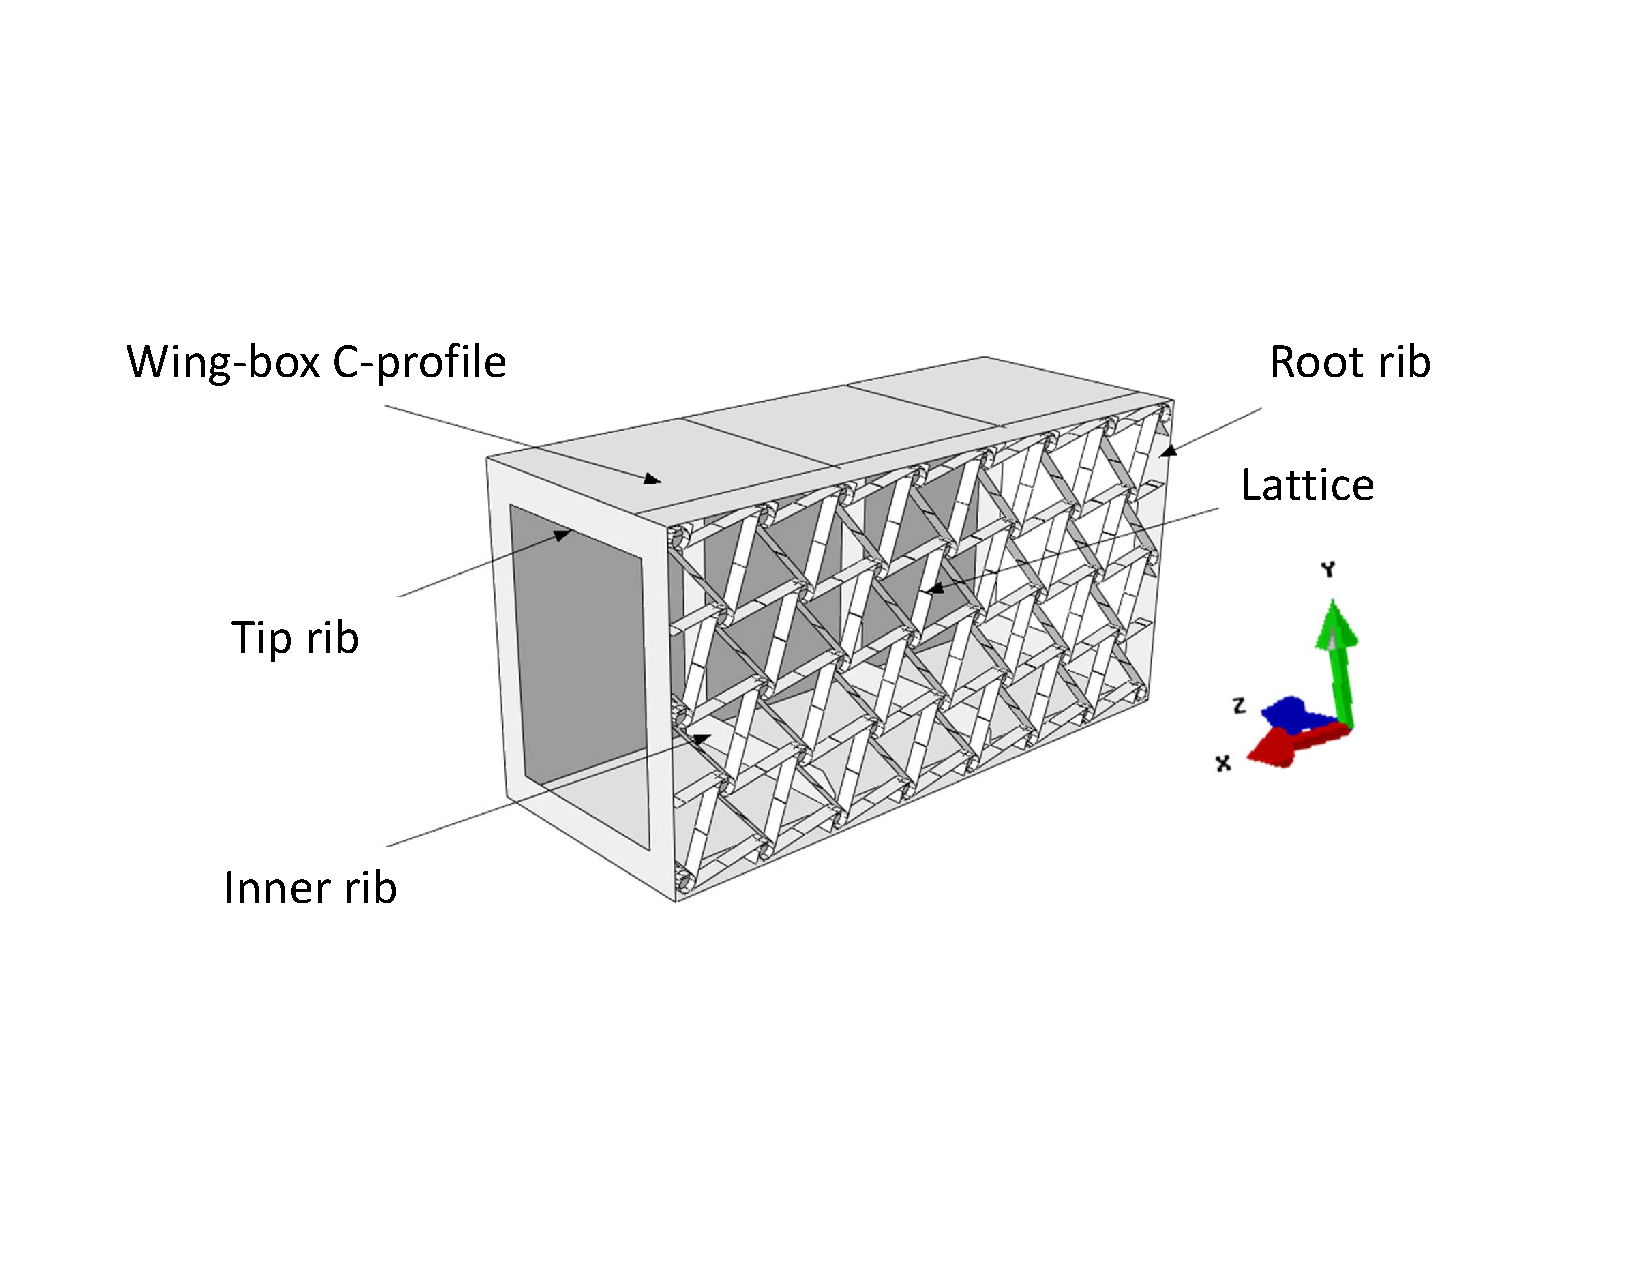
\includegraphics[width=0.8 \textwidth]{model/all-assembly}
  \caption[General assembly configuration for the computational model]{General assembly configuration for the computational model. The different parts for the general configuration include the wing-box profile, the lattice and the pair of ribs located at the tip and the root of the wing-box.}\label{fig:all-assembly}
\end{figure}

\subsection{Sub-parts and parametrization of the model} \label{subsec:parametrization_Model}

\subsubsection{Lattice of chiral elements} \label{subsubsec:lattice_Parametrization}

The model of the lattice structure is constituted of a series of interconnected lattices and nodes. An overview of the corresponding part can be seen in Figure \ref{fig:lattice}. The lattice structure is divided in an integer number of unit cells in the longitudinal (spanwise) and transversal directions. These parameters are identified with the variables $N$ and $M$ for the longitudinal and transversal directions, respectively. In Figure \ref{fig:lattice-NandM}, these internal division can be understood.

Furthermore, the internal geometry in the chiral lattices is determined by a number of parameters: the thickness $t_{\mathrm{chiral}}$, the ligament eccentricity $e_{\mathrm{chiral}}$, the ligament half length $L_{\mathrm{chiral}}$, the lattice node depth $B_{\mathrm{chiral}}$ and the lattice node radius $r_{\mathrm{chiral}}$. The geometrical meaning of these variables can be seen in Figure \ref{fig:lattice-internalParameters}. The thickness $t_{\mathrm{chiral}}$ applies for both the ligaments and the lattice nodes geometries. The eccentricity $e_{\mathrm{chiral}}$ will be expressed as the dimensionless parameter $\hat{e}_{\mathrm{chiral}}$ which is obtained from $\hat{e}_{\mathrm{chiral}} = e_{\mathrm{chiral}} / B_{\mathrm{chiral}}$.

In the sketch shown in Figure \ref{fig:lattice-internalParameters} an additional dimension variable appears, the ligament eccentricity radius $R_{\mathrm{chiral}}$ which is dependent on the ligament eccentricity $e_{\mathrm{chiral}}$ and the lattice node depth $B_{\mathrm{chiral}}$ as shown in Equation \ref{eq:RforLattice}.

A summary of all the parameters introduced to characterize the chiral lattice structure together with their units and nominal values is shown in Table \ref{tab:parameters_lattice}.

\begin{equation}\label{eq:RforLattice}
  R = \frac{e_{\mathrm{chiral}}^2 + \frac{B_{\mathrm{chiral}}^2}{4}}{2e_{\mathrm{chiral}}}
\end{equation}

\begin{figure}[!htpb]
  \centering
  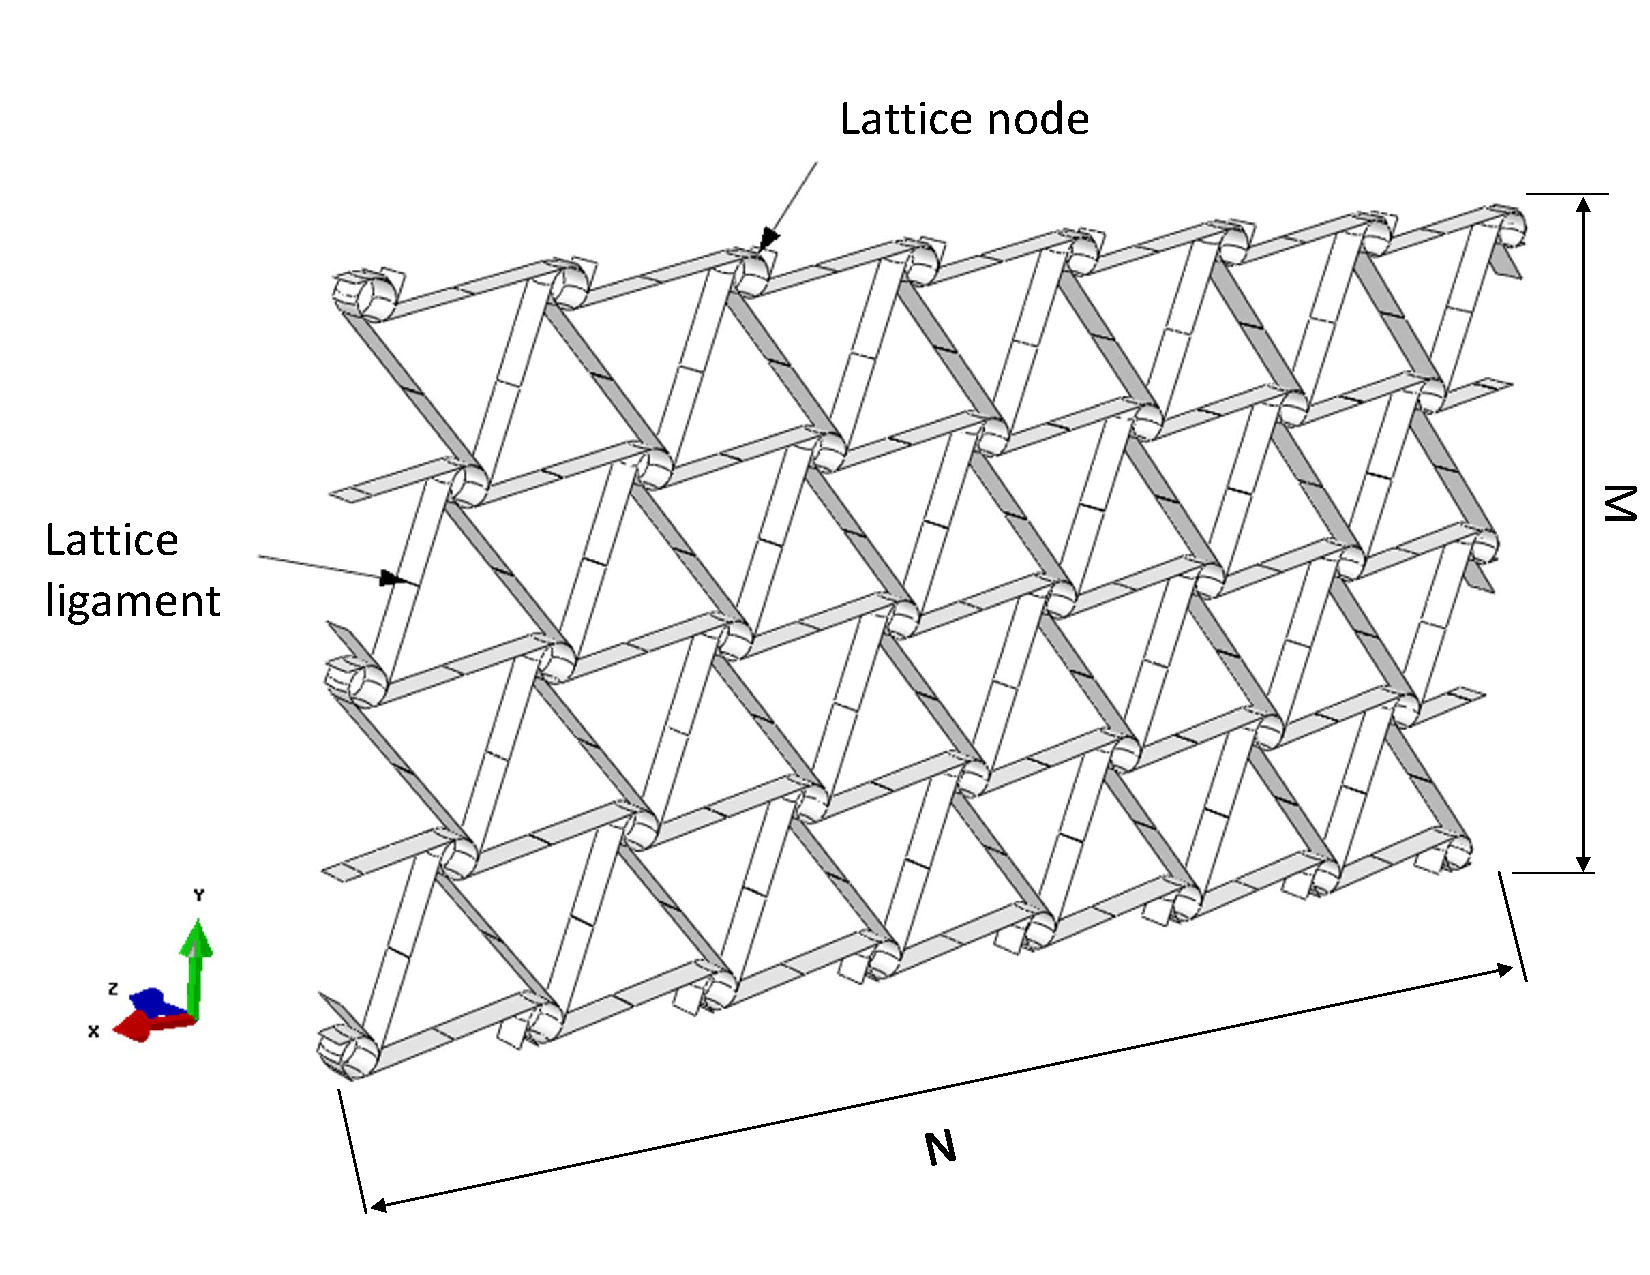
\includegraphics[width=0.8 \textwidth]{model/lattice}
  \caption[Overview of the chiral lattice part]{Overview of the chiral lattice part. The parameters $N$ and $M$ represent the number of unit cells in the longitudinal (spanwise) and transversal directions, respectively.}\label{fig:lattice}
\end{figure}

\begin{figure}[!htpb]
  \centering
  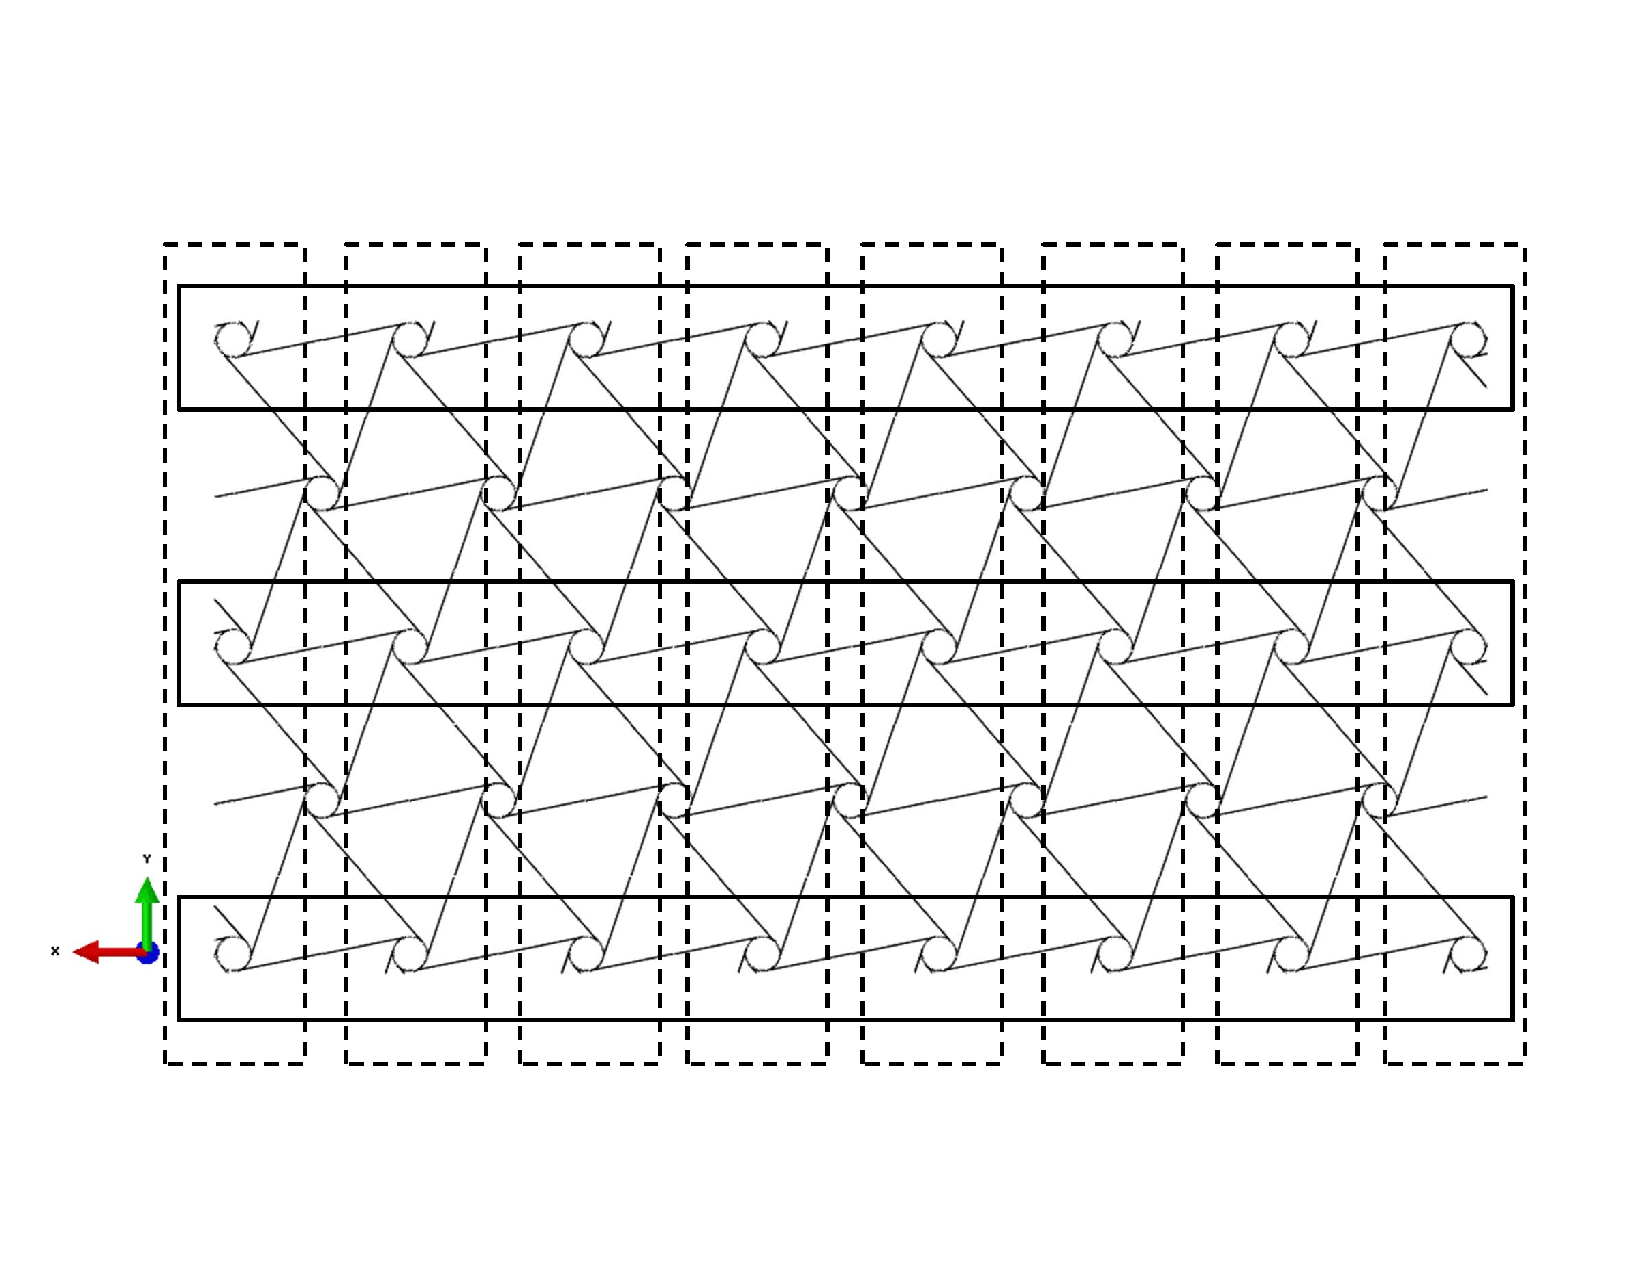
\includegraphics[width=0.8 \textwidth]{model/lattice-NandM}
  \caption[Division of the lattice structure in cell units]{Division of the lattice structure in cell units. The sketch shows a lattice with $N = 8$ and $M = 3$. The set of horizontal rectangles represent each of the transversal $M$ divisions while the set of vertical rectangles correspond to each of the $N$ longitudinal divisions.}\label{fig:lattice-NandM}
\end{figure}

\begin{figure}[!htpb]
  \centering
  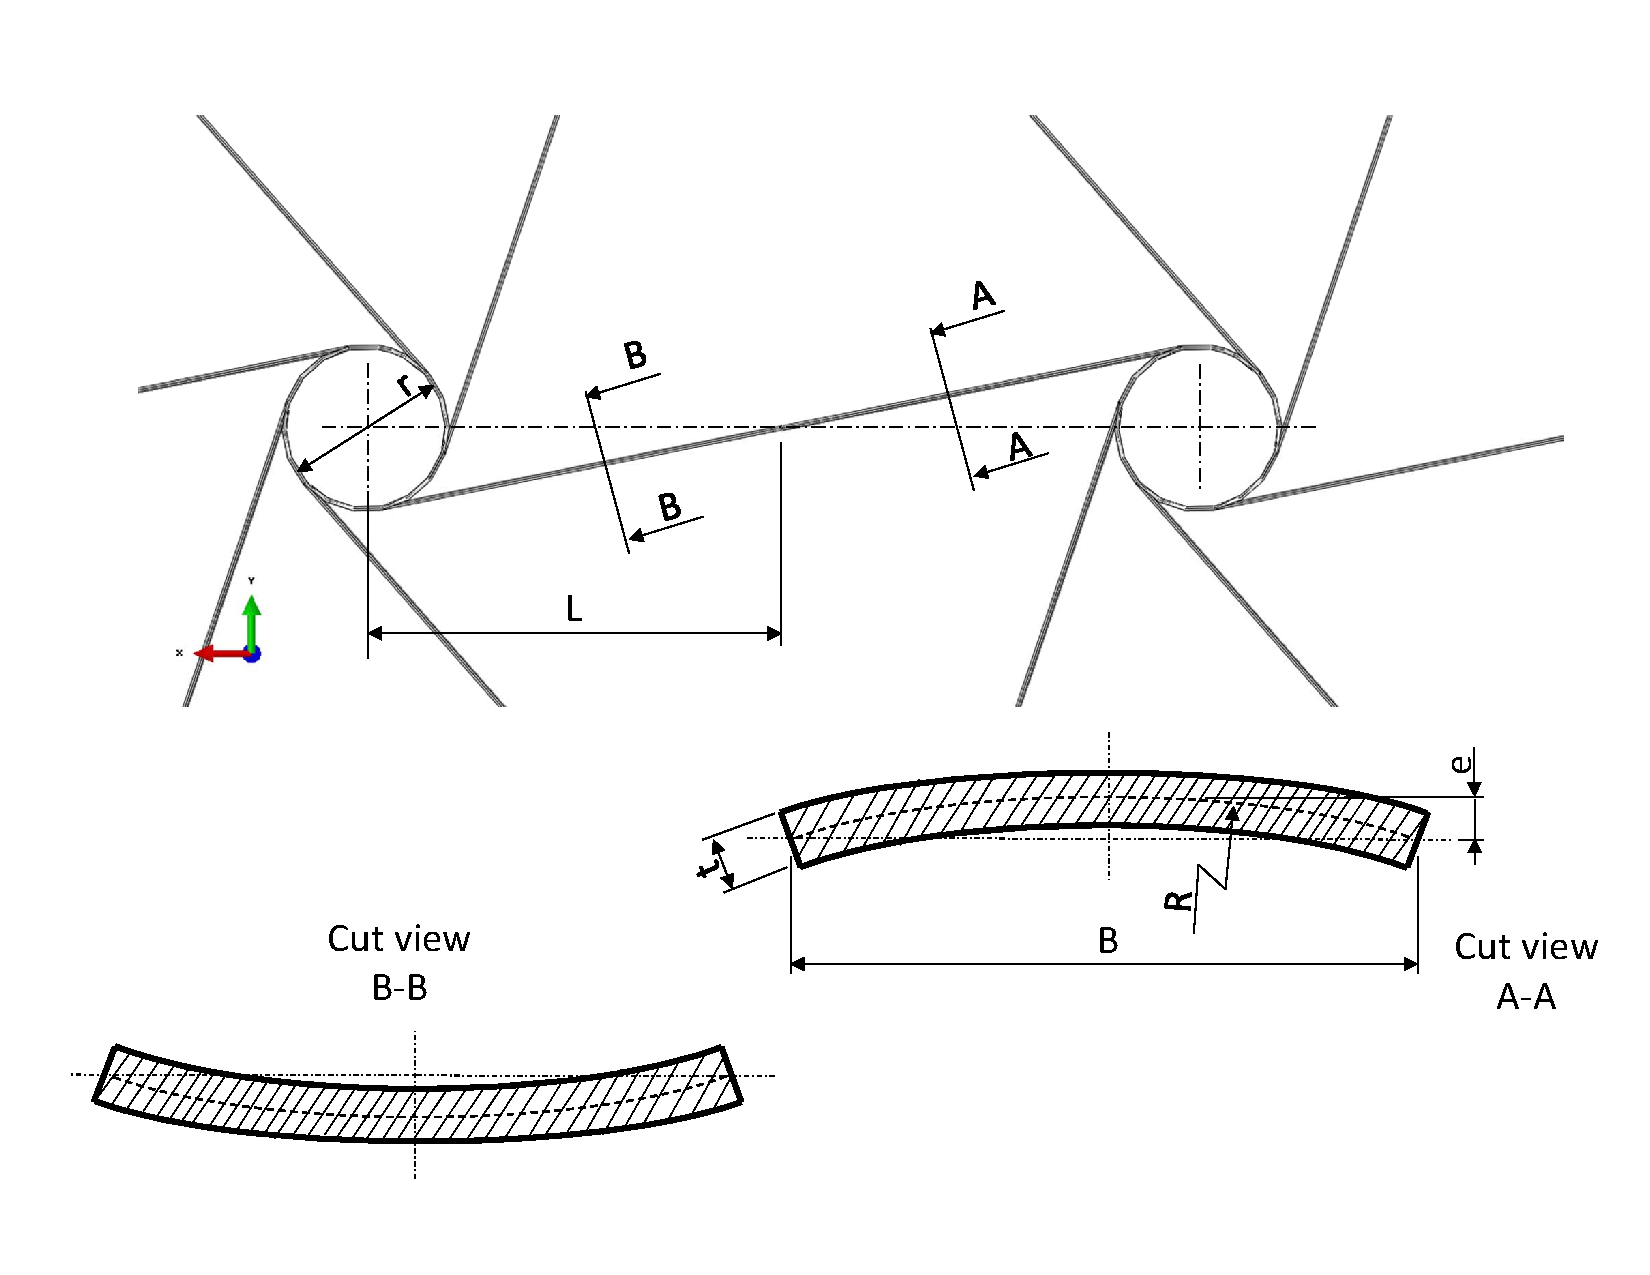
\includegraphics[width=0.8 \textwidth]{model/lattice-internalParameters}
  \caption[Internal parameters of the chiral lattice structure]{Internal parameters of the chiral lattice structure. The geometry is characterized by the the ligament eccentricity $e_{\mathrm{chiral}}$, the ligament half length $L_{\mathrm{chiral}}$, the lattice node depth $B_{\mathrm{chiral}}$, the lattice node radius $r_{\mathrm{chiral}}$ and the thickness $t_{\mathrm{chiral}}$.}\label{fig:lattice-internalParameters}
\end{figure}

\begin{table}[!htpb]
\centering
\begin{tabular}{|l|lll|}
\hline
\textbf{Parameter} & \multicolumn{1}{l|}{\textbf{Symbol}} & \multicolumn{1}{l|}{\textbf{Units}} & \textbf{Nominal value} \\ \hline \hline
{\textbf{Dimensions}} &  &  &  \\ \hline
Number of unit cells in spanwise direction & \multicolumn{1}{l|}{$N$} & \multicolumn{1}{l|}{} & 8 \\ \hline
Number of unit cells in transversal direction & \multicolumn{1}{l|}{$M$} & \multicolumn{1}{l|}{} & 3 \\ \hline
Dimensionless ligament eccentricity (e/B) & \multicolumn{1}{l|}{$\hat{e}_{\mathrm{chiral}}$} & \multicolumn{1}{l|}{} & 0.01 \\ \hline
Node radius & \multicolumn{1}{l|}{$r_{\mathrm{chiral}}$} & \multicolumn{1}{l|}{mm} & 10 \\ \hline
Ligament eccentricity radius & \multicolumn{1}{l|}{$R_{\mathrm{chiral}}$} & \multicolumn{1}{l|}{mm} & 250.1 \\ \hline
Node depth & \multicolumn{1}{l|}{$B_{\mathrm{chiral}}$} & \multicolumn{1}{l|}{mm} & 20 \\ \hline
Ligament half length & \multicolumn{1}{l|}{$L_{\mathrm{chiral}}$} & \multicolumn{1}{l|}{mm} & 50 \\ \hline \hline
{\textbf{Material (ABS)}} &  &  &  \\ \hline
Young's modulus & \multicolumn{1}{l|}{$E_{\mathrm{chiral}}$} & \multicolumn{1}{l|}{N/mm$^2$} & 3100 \\ \hline
Poisson's ratio & \multicolumn{1}{l|}{$\nu_{\mathrm{chiral}}$} & \multicolumn{1}{l|}{} & 0.3 \\ \hline
\end{tabular}
\caption[Parameters used for the lattice model]{Parameters used for the lattice model. The mechanical properties of the material used correspond to ABS, which is a common thermoplastic polymer.}
\label{tab:parameters_lattice}
\end{table}

%This is like if it was a new section inside of this section
\clearpage
\subsubsection{Lattice nodes rigid body modeling} \label{subsubsec:latticeNodesRigid_Parametrization}

The lattice nodes is one of the essential parts of the lattice of chiral elements. These are allow to freely rotate around its own axis. For the modeling, they are assumed to behave like a rigid body. In Figure \ref{fig:closeLookToLatticeNodes}, a closer look to the chiral nodes can be seen, showing two different approaches to manufacture a node that would behave like a rigid body compared with the rest of the structure.

\begin{figure}[!htpb]
  \centering
  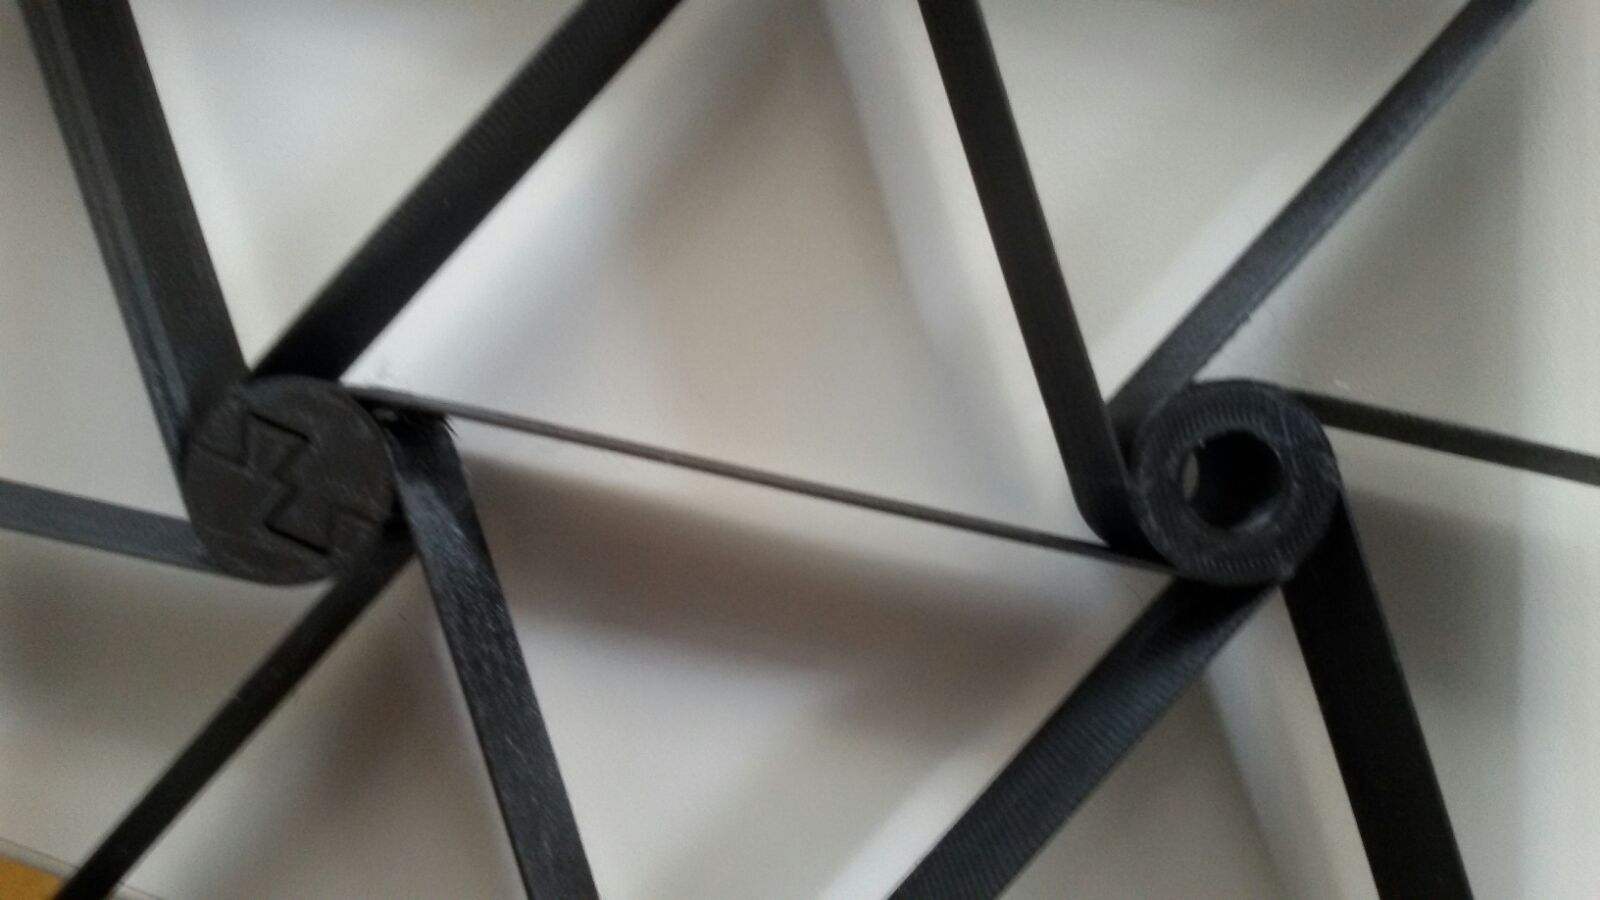
\includegraphics[width=0.8 \textwidth]{model/closeLookToLatticeNodes-tobeimproved}
  \caption[Pictured of the manufactured chiral lattice nodes]{Pictured of the manufactured chiral lattice nodes. The figures shows two different approaches followed to manufacture the nodes. The one on the right was the standard one showing a cylinder with a thickness bigger than the thickness of the chiral ligaments $t_{\mathrm{node}} \gg t_{\mathrm{ligaments}}$. On the left, an alternative approach is followed in order to allow the assembly of the chiral lattice that is not manufactured as a unique piece. \cite{Vincenz2017}}\label{fig:closeLookToLatticeNodes}
\end{figure}

In the Abaqus model, different approaches were followed to create this element of the chiral lattice. The chiral lattice node is build together with the lattice ligaments, as a single part having homogeneous mechanical properties and thickness. Therefore, it is necessary to ensure the rigid body properties by other means.

The first approach was to create a coupling condition using Abaqus corresponding module. In particular, a kinematic coupling was establish. Kinematic coupling constrains the motion of one or more coupling nodes, also called slave node or nodes, to the rigid body motion of a reference node, also called master node. They are imposed by eliminating degrees of freedom at the coupling nodes. In Figure \ref{fig:kinematicCoupling}, an example of a kinematic coupling can be seen.

\begin{figure}[!htpb]
  \centering
  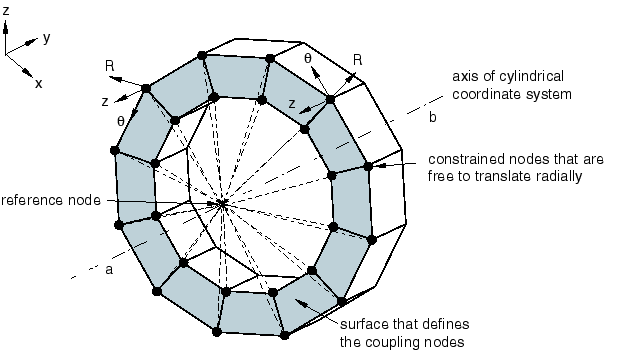
\includegraphics[width=0.8 \textwidth]{model/pcoupling-kinematic}
  \caption[Kinematic coupling constraint]{Kinematic coupling constraint. The sketch illustrates the use of a kinematic coupling constraint to prescribe a twisting motion to a model without constraining the radial motion. In this case, a local cylindrical reference system is used and the constrained nodes have two degrees of freedom coupled to those of the reference node, the angular position $\theta$ and the position along the $z$ axis. The coupling nodes are therefore free to translate radially, varying $R$. \cite{Abaqus}}\label{fig:kinematicCoupling}
\end{figure}

For the considered case, the coupling nodes are those mesh nodes located faces of the lattice node and the master node is the reference point located in the center of the lattice node. In order to achieve the rigid solid behavior, all the degrees of freedom were coupled except from the translation displacements in the plane where the chiral lattice is contained, i.e. the translational displacement $U_1$ and $U_2$ of the plane $X-Y$. In Figure \ref{fig:couplingThroughRF} an overview of this coupling condition can be viewed.

\begin{figure}[!htpb]
  \centering
  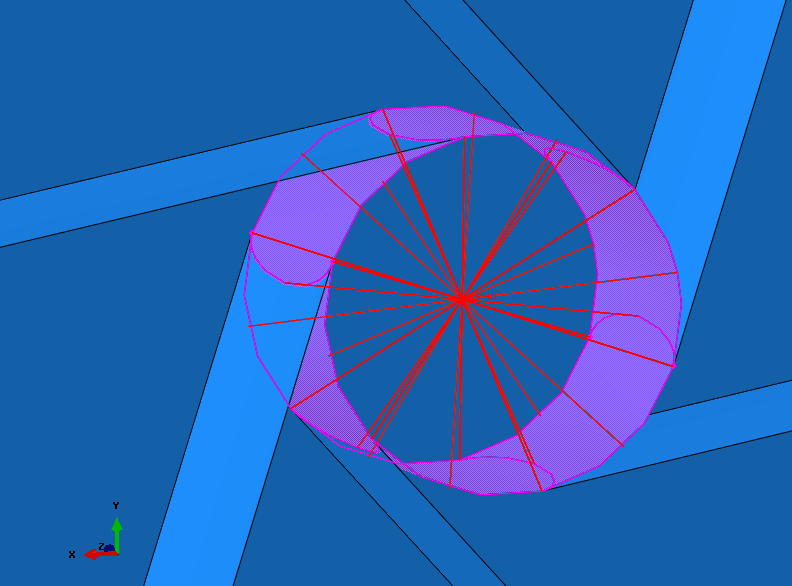
\includegraphics[width=0.8 \textwidth]{model/couplingThroughRF}
  \caption[Overview of the elements that are involved in the coupling condition at the lattice nodes]{Overview of the elements that are involved in the coupling condition at the lattice nodes. The coupling condition was defined in between the mesh nodes located in the faces of the lattince node and a reference point located in the middle. All the degrees of fredom were linked except from the translation displacements in the plane where the chiral lattice is contained, i.e. the translational displacement $U_1$ and $U_2$ of the plane $X-Y$.}\label{fig:couplingThroughRF}
\end{figure}

Another approach consisted in inserting an addition part inside the lattice nodes to add rigidity to the element. The proposed design of such a part, which will be referred as tyre from now on, can be seen in Figure \ref{fig:tyre-part}. The internal dimensions of this element are shown in Figure \ref{fig:tyre-internalParameters}. This dimensions were dependent on parameters of the chiral lattice. In other words, the thickness of the tyre was equal to that of the chiral lattice $r_{\mathrm{tyre}} = r_{\mathrm{chiral}}$ and the same occurred for the height $B_{\mathrm{tyre}}$ and the radius $r_{\mathrm{tyre}}$ which were $r_{\mathrm{tyre}} = r_{\mathrm{chiral}}$ and $B_{\mathrm{tyre}} = B_{\mathrm{chiral}}$. The added rigidity was obtained as a result of considering a different material for the tyre such that the Young's modulus of the two parts verify the condition $E_{\mathrm{tyre}} \gg E_{\mathrm{chiral}}$. Once, the connection was completed, the resulting merged part looked as shown in Figure \ref{fig:tyre-connection}.

\begin{figure}[!htpb]
  \centering
  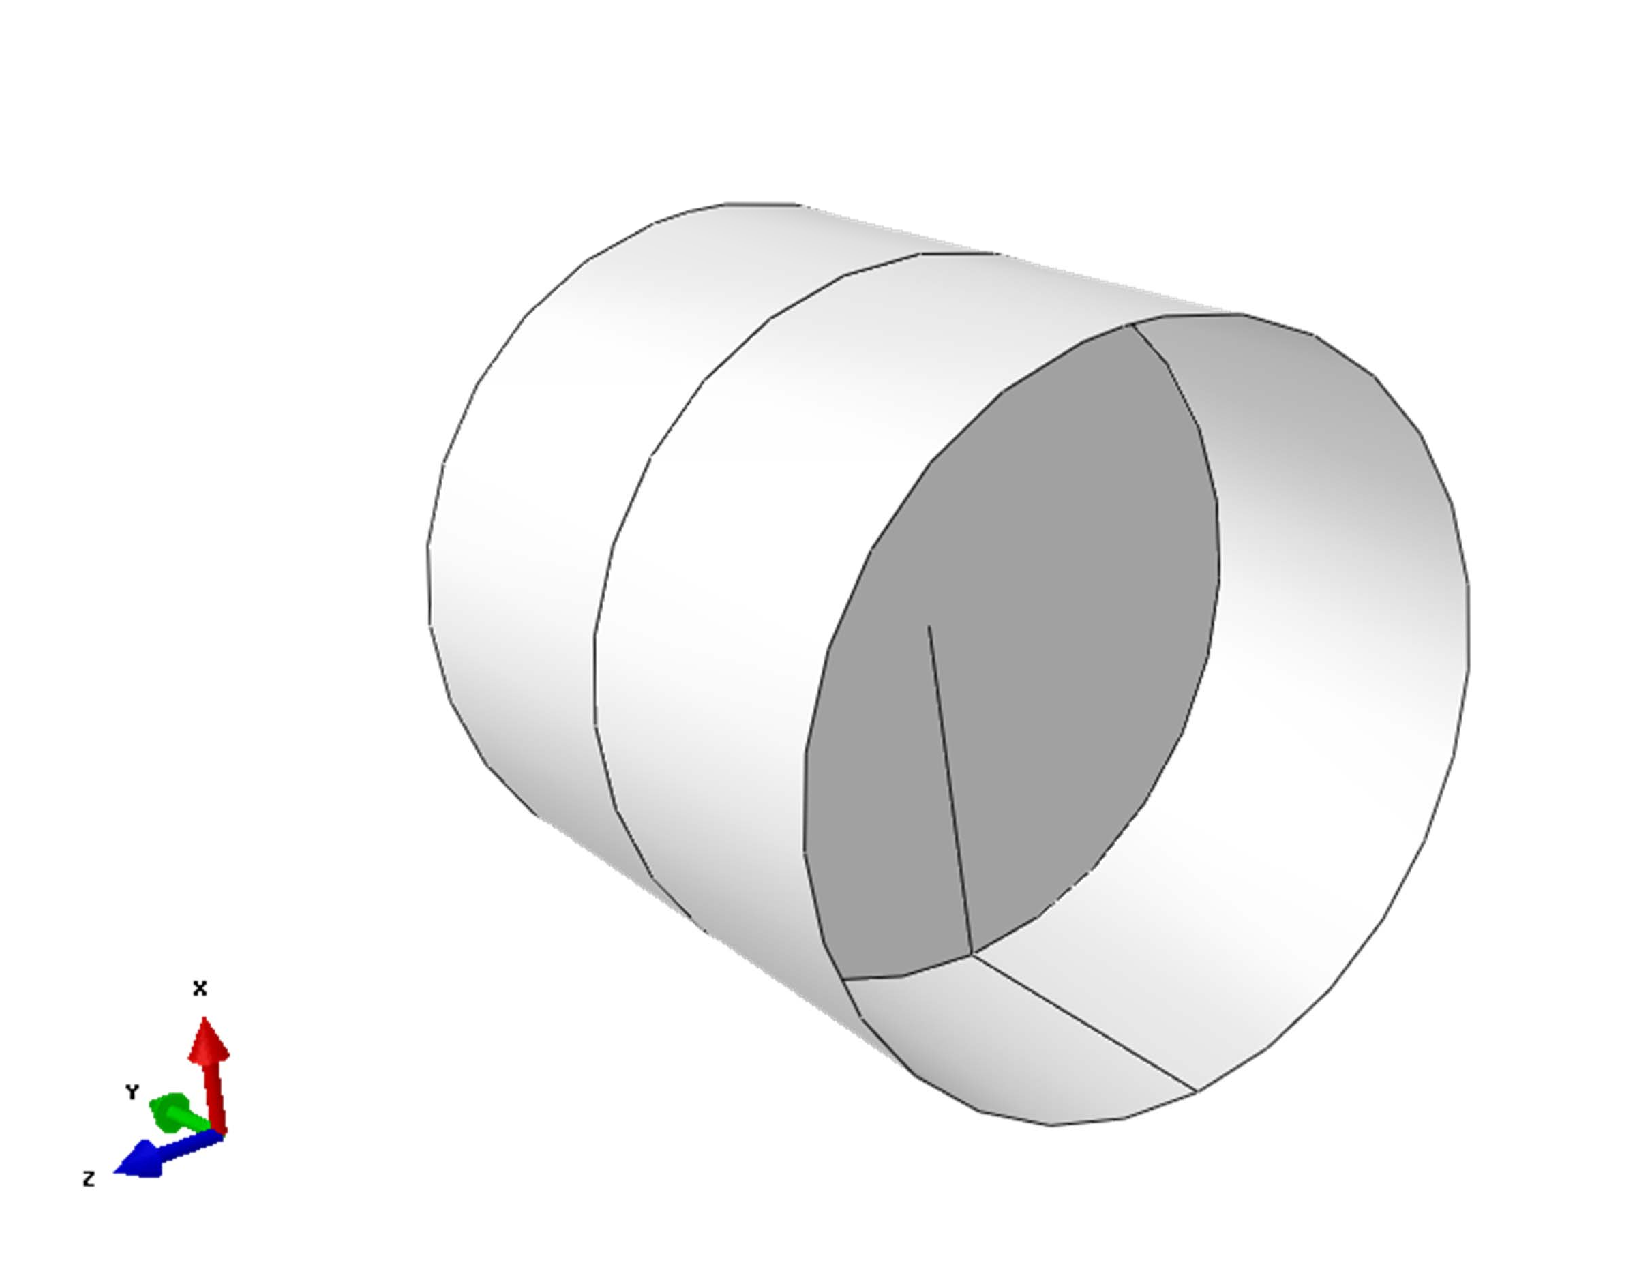
\includegraphics[width=0.8 \textwidth]{model/tyre-part}
  \caption[Overview of the tyre part]{Overview of the tyre part.}\label{fig:tyre-part}
\end{figure}

\begin{figure}[!htpb]
  \centering
  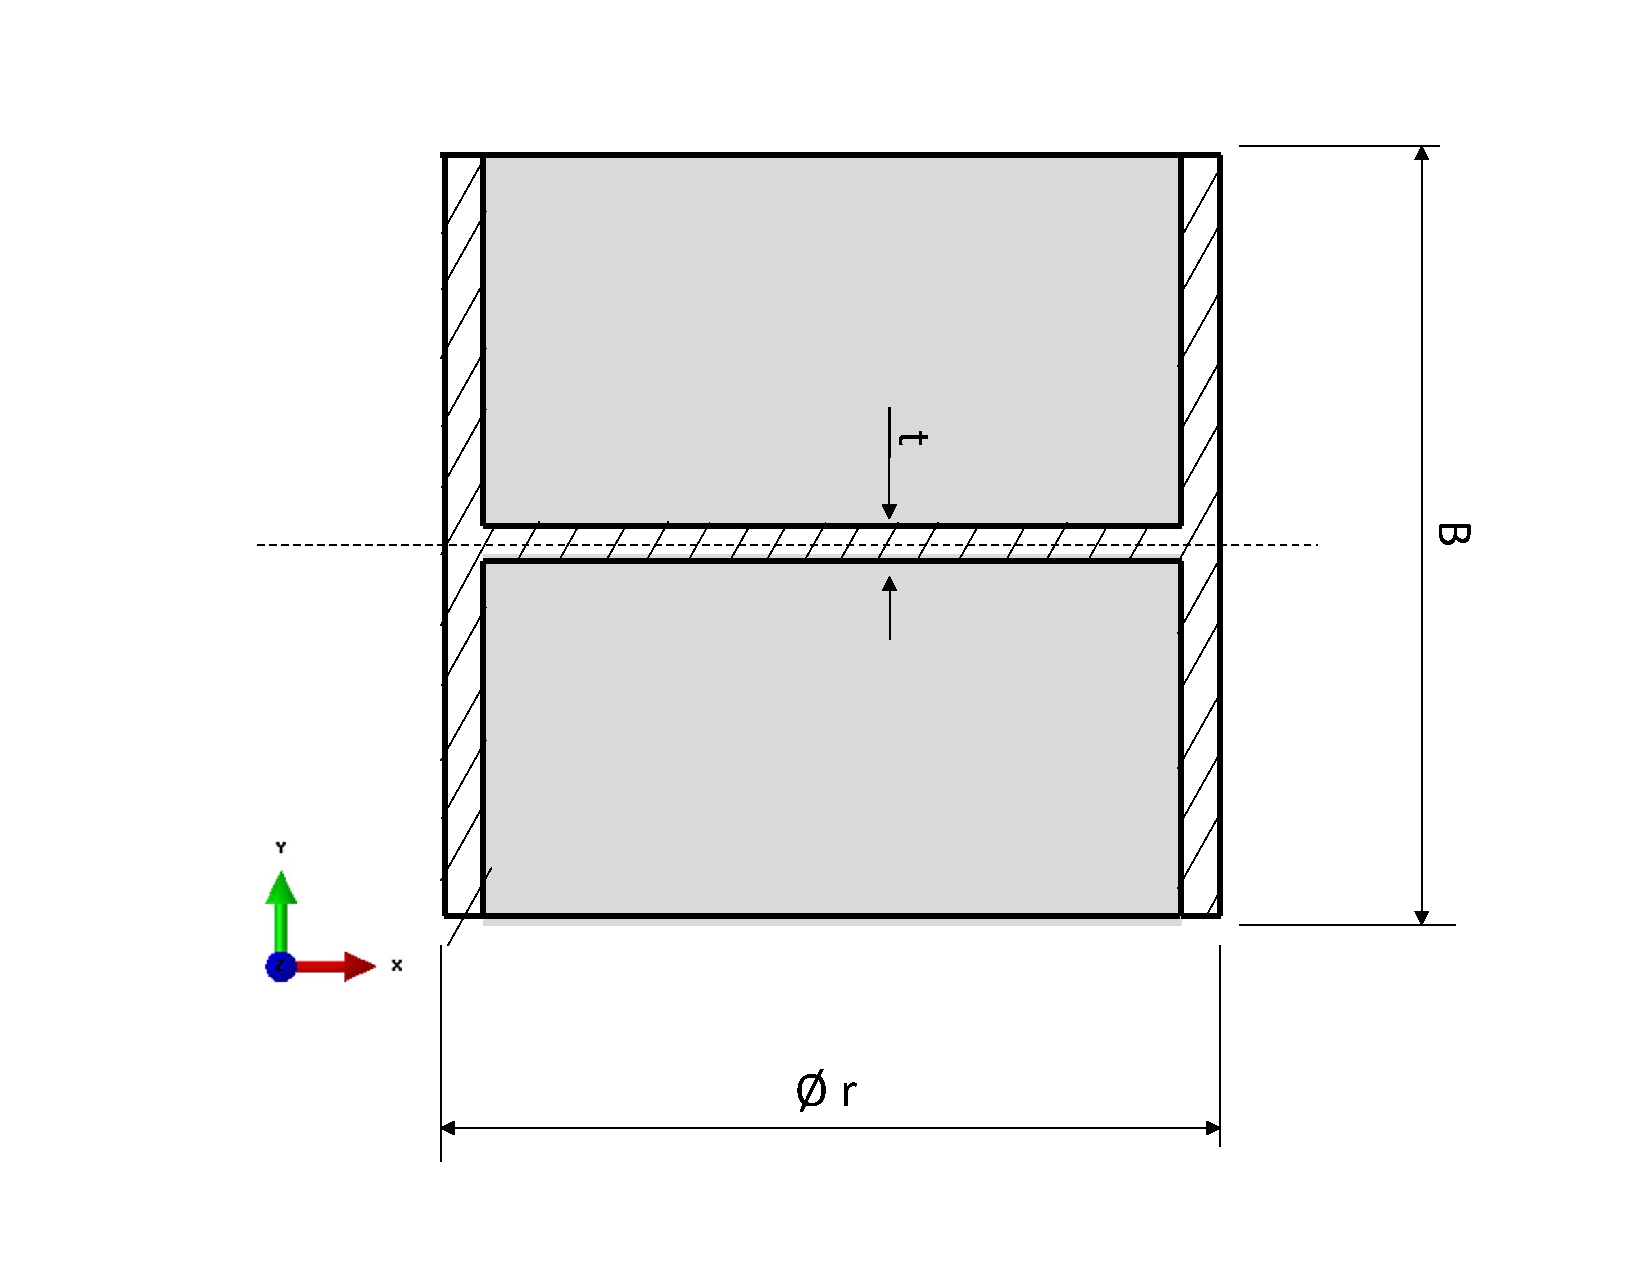
\includegraphics[width=0.8 \textwidth]{model/tyre-internalParameters}
  \caption[Internal parameters of the tyre part]{Internal parameters of the tyre part. The sketch shows a transversal cut to the part. The tyre is characterized by the radius $r_{\mathrm{tyre}}$, the height $B_{\mathrm{tyre}}$ and the thickness $t_{\mathrm{tyre}}$. All this parameters were equal to the corresponding ones in the lattice nodes, therefore: $r_{\mathrm{tyre}} = r_{\mathrm{chiral}}$, $B_{\mathrm{tyre}} = B_{\mathrm{chiral}}$ and $t_{\mathrm{tyre}} = t_{\mathrm{chiral}}$.}\label{fig:tyre-internalParameters}
\end{figure}

\begin{figure}[!htpb]
  \centering
  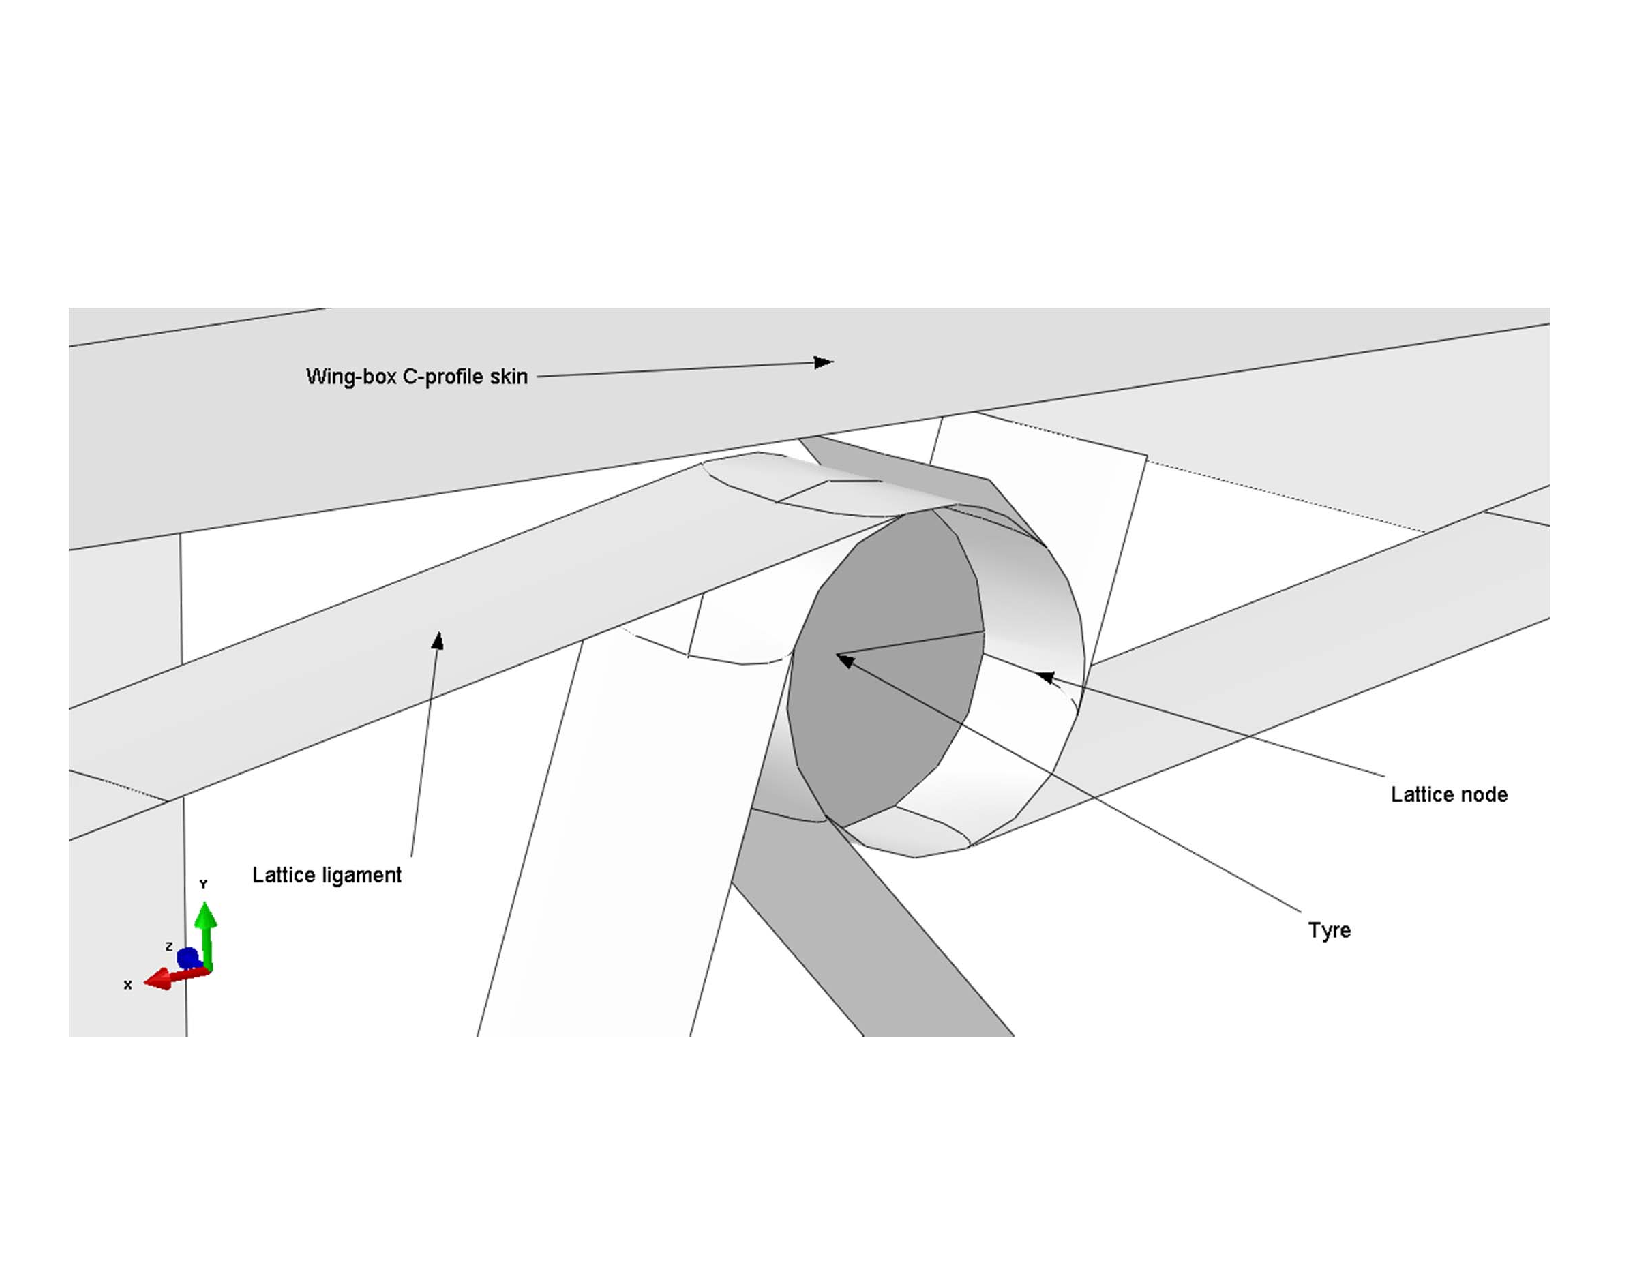
\includegraphics[width=0.8 \textwidth]{model/tyre-connection}
  \caption[Overview of the connection between tyre and lattice node]{Overview of the connection between tyre and lattice node. The tyre will be embed inside the lattice node.}\label{fig:tyre-connection}
\end{figure}

\clearpage
\subsubsection{Wing-box in C-profile} \label{subsubsec:wingBox_Parametrization}

%Description of the wing box
The model of the wing-box consisted on a beam with open C profile. The length $L_{\mathrm{box}}$ and height $H_{\mathrm{box}}$ of the part were determined from those of the lattice of chiral elements. Therefore, the tailorable parameters for this part are the width $W_{\mathrm{box}}$, the thickness $t_{\mathrm{box}}$ and the mechanical properties $E_{\mathrm{box}}$ and $\nu_{\mathrm{box}}$ of the material used. The value of the Wing-box height $H_{\mathrm{box}}$ and the wing-box length $L_{\mathrm{box}}$ are not independent but are calculated based on the transversal and longitudinal dimensions of the chiral lattice structure, respectively.

\begin{figure}[!htpb]
  \centering
  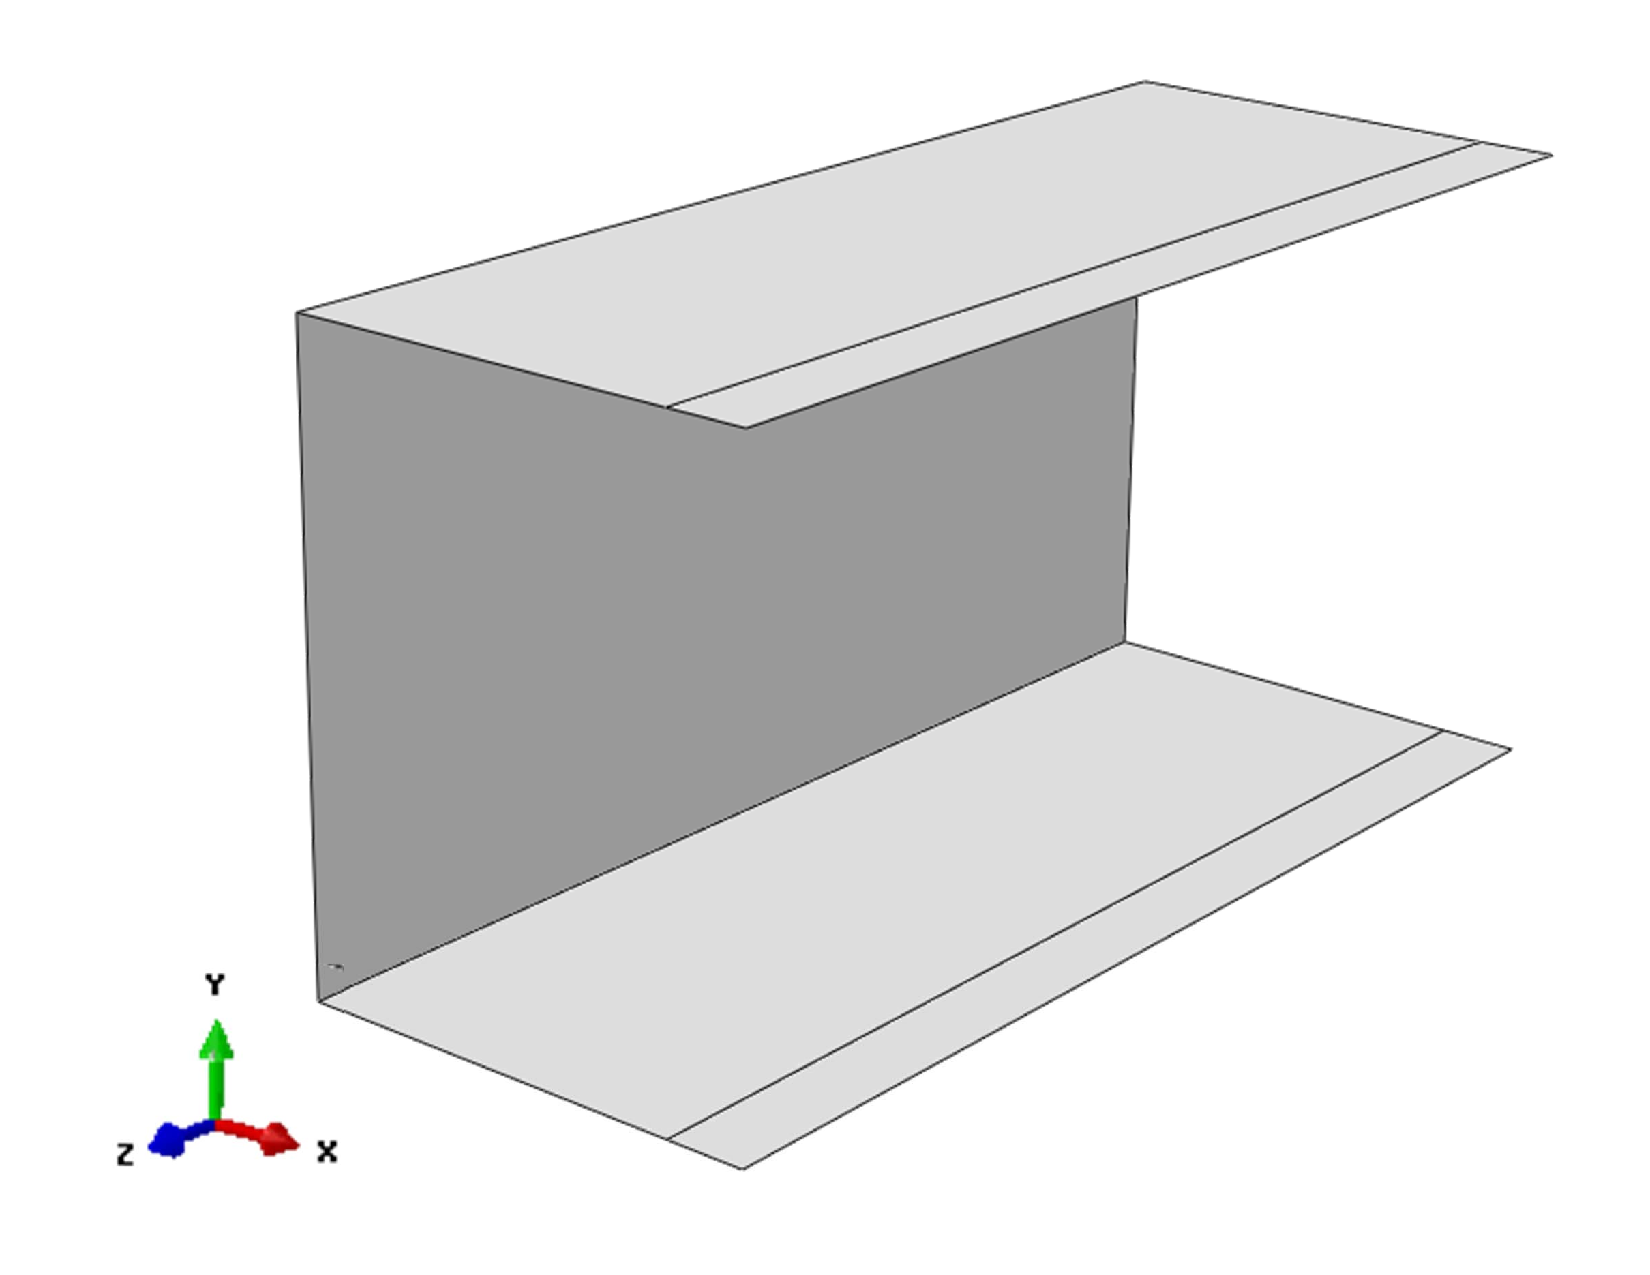
\includegraphics[width=0.8 \textwidth]{model/wing-box}
  \caption[Overview of the wing-box in C-profile part]{Overview of the wing-box in C-profile part}\label{fig:wing-box}
\end{figure}

In the sketch shown in Figure \ref{fig:wing-box-internalParameters} it is possible see the geometrical meaning of the parameters introduced in the previous paragraph. Additionally, the Table \ref{tab:parameters_wing-box} shows its units and nominal values.

\begin{figure}[!htpb]
  \centering
  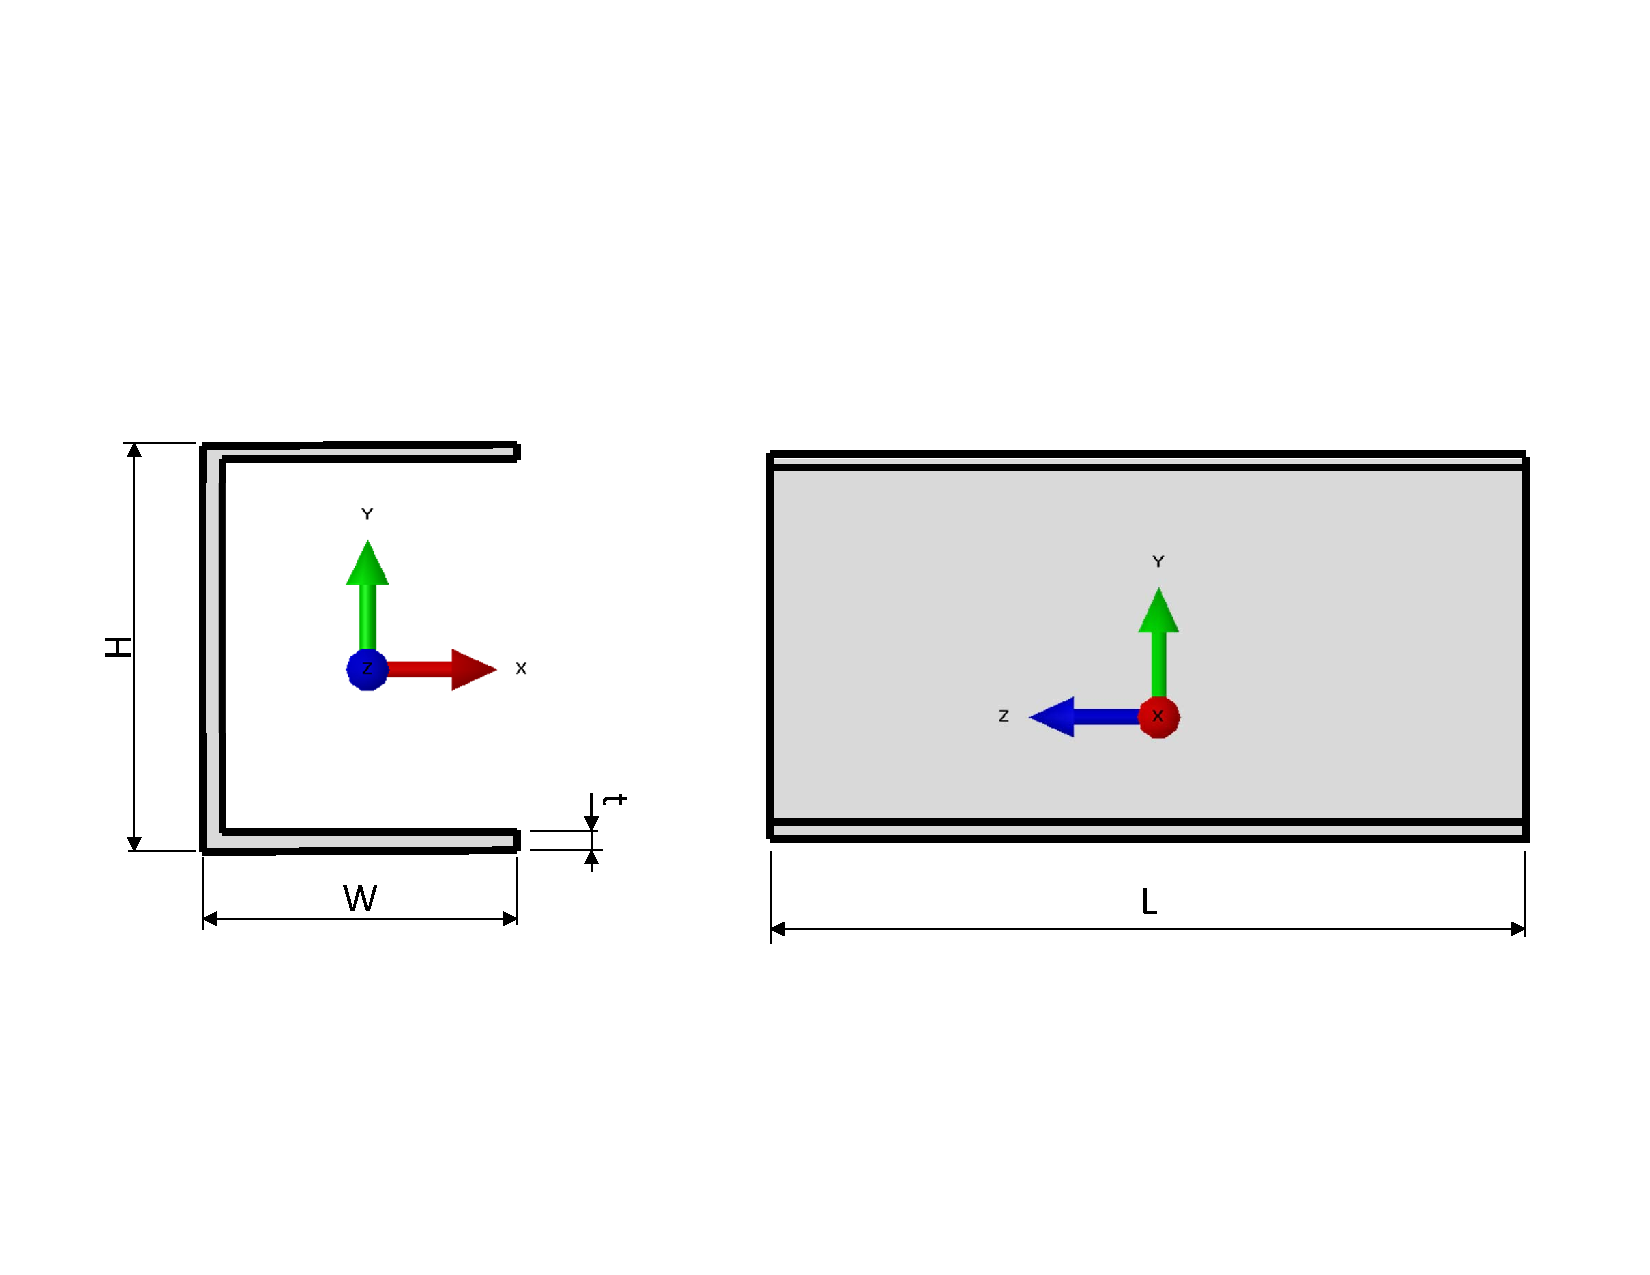
\includegraphics[width=0.8 \textwidth]{model/wing-box-internalParameters}
  \caption[Internal parameters of the wing-box in C-profile part]{Internal parameters of the wing-box C-profile part. The geometry of the part is determined by the length $L_{\mathrm{box}}$, height $H_{\mathrm{box}}$ and the width $W_{\mathrm{box}}$. Additionally, the thickness $t_{\mathrm{box}}$ is measured in the $z$ direction.}\label{fig:wing-box-internalParameters}
\end{figure}

\begin{table}[!htpb]
\centering
\begin{tabular}{|l|lll|}
\hline
\textbf{Parameter} & \multicolumn{1}{l|}{\textbf{Symbol}} & \multicolumn{1}{l|}{\textbf{Units}} & \textbf{Nominal value} \\ \hline \hline
{\textbf{Dimensions}} &  &  &  \\ \hline
Wing-box height & \multicolumn{1}{l|}{$H_{\mathrm{box}}$} & \multicolumn{1}{l|}{mm} & 383.27 \\ \hline
Wing-box length & \multicolumn{1}{l|}{$L_{\mathrm{box}}$} & \multicolumn{1}{l|}{mm} & 743.86 \\ \hline
Wing-box width & \multicolumn{1}{l|}{$W_{\mathrm{box}}$} & \multicolumn{1}{l|}{mm} & 300 \\ \hline
Wing-box thickness & \multicolumn{1}{l|}{$t_{\mathrm{box}}$} & \multicolumn{1}{l|}{mm} & 0.8 \\ \hline \hline
{\textbf{Material (Aluminum)}} &  &  &  \\ \hline
Young's modulus & \multicolumn{1}{l|}{$E_{\mathrm{box}}$} & \multicolumn{1}{l|}{N/mm$^2$} & 69000 \\ \hline
Poisson's ratio & \multicolumn{1}{l|}{$\nu_{\mathrm{box}}$} & \multicolumn{1}{l|}{} & 0.3269 \\ \hline
\end{tabular}
\caption[Parameters used for the wing-box in C-profile model]{Parameters used for the wing-box in C-profile model. The mechanical properties of the material used correspond to standard aluminum. The value of the wing-box height $H_{\mathrm{box}}$ and the wing-box length $L_{\mathrm{box}}$ are not independent but are calculated based on the transversal and longitudinal dimensions of the chiral lattice structure, respectively.}
\label{tab:parameters_wing-box}
\end{table}

\clearpage
\subsubsection{Ribs} \label{subsubsec:Ribs_Parametrization}

As it was shown in Figure \ref{fig:all-assembly}, there are two possible ribs that can be added to the model assembly. This will add rigidity to the wing-box. The ribs located at the tip and at the root will have a closed section, similar to a frame with width $A_{\mathrm{rib}}$. The width $W_{\mathrm{rib,close}}$ and the height $H_{\mathrm{rib}}$ will be equal to the wing-box width $W_{\mathrm{box}}$ and to the chiral lattice structure height, respectively. The thickness will be $t_{\mathrm{rib}}$.

The inner ribs will present an open section with same height $H_{\mathrm{rib}}$ and thickness $t_{\mathrm{rib}}$ as the closed configuration but different width $W_{\mathrm{rib,open}}$. The value of $W_{\mathrm{rib,open}}$ is calculated as follows:
$$
W_{\mathrm{rib,open}} = B_{\mathrm{chiral}} + W_{\mathrm{rib,close}} + d_{\mathrm{chiral-rib}}
$$
where $d_{\mathrm{chiral-rib}}$ represents the gap between the right edges of the inner rib and the lattice chiral structure. This gap ensures that there are not any interferences in between the rib and the lattice chiral structure. The value of this parameter was set to $d_{\mathrm{chiral-rib}} = 20$mm.

\begin{figure}[!htpb]
  \centering
  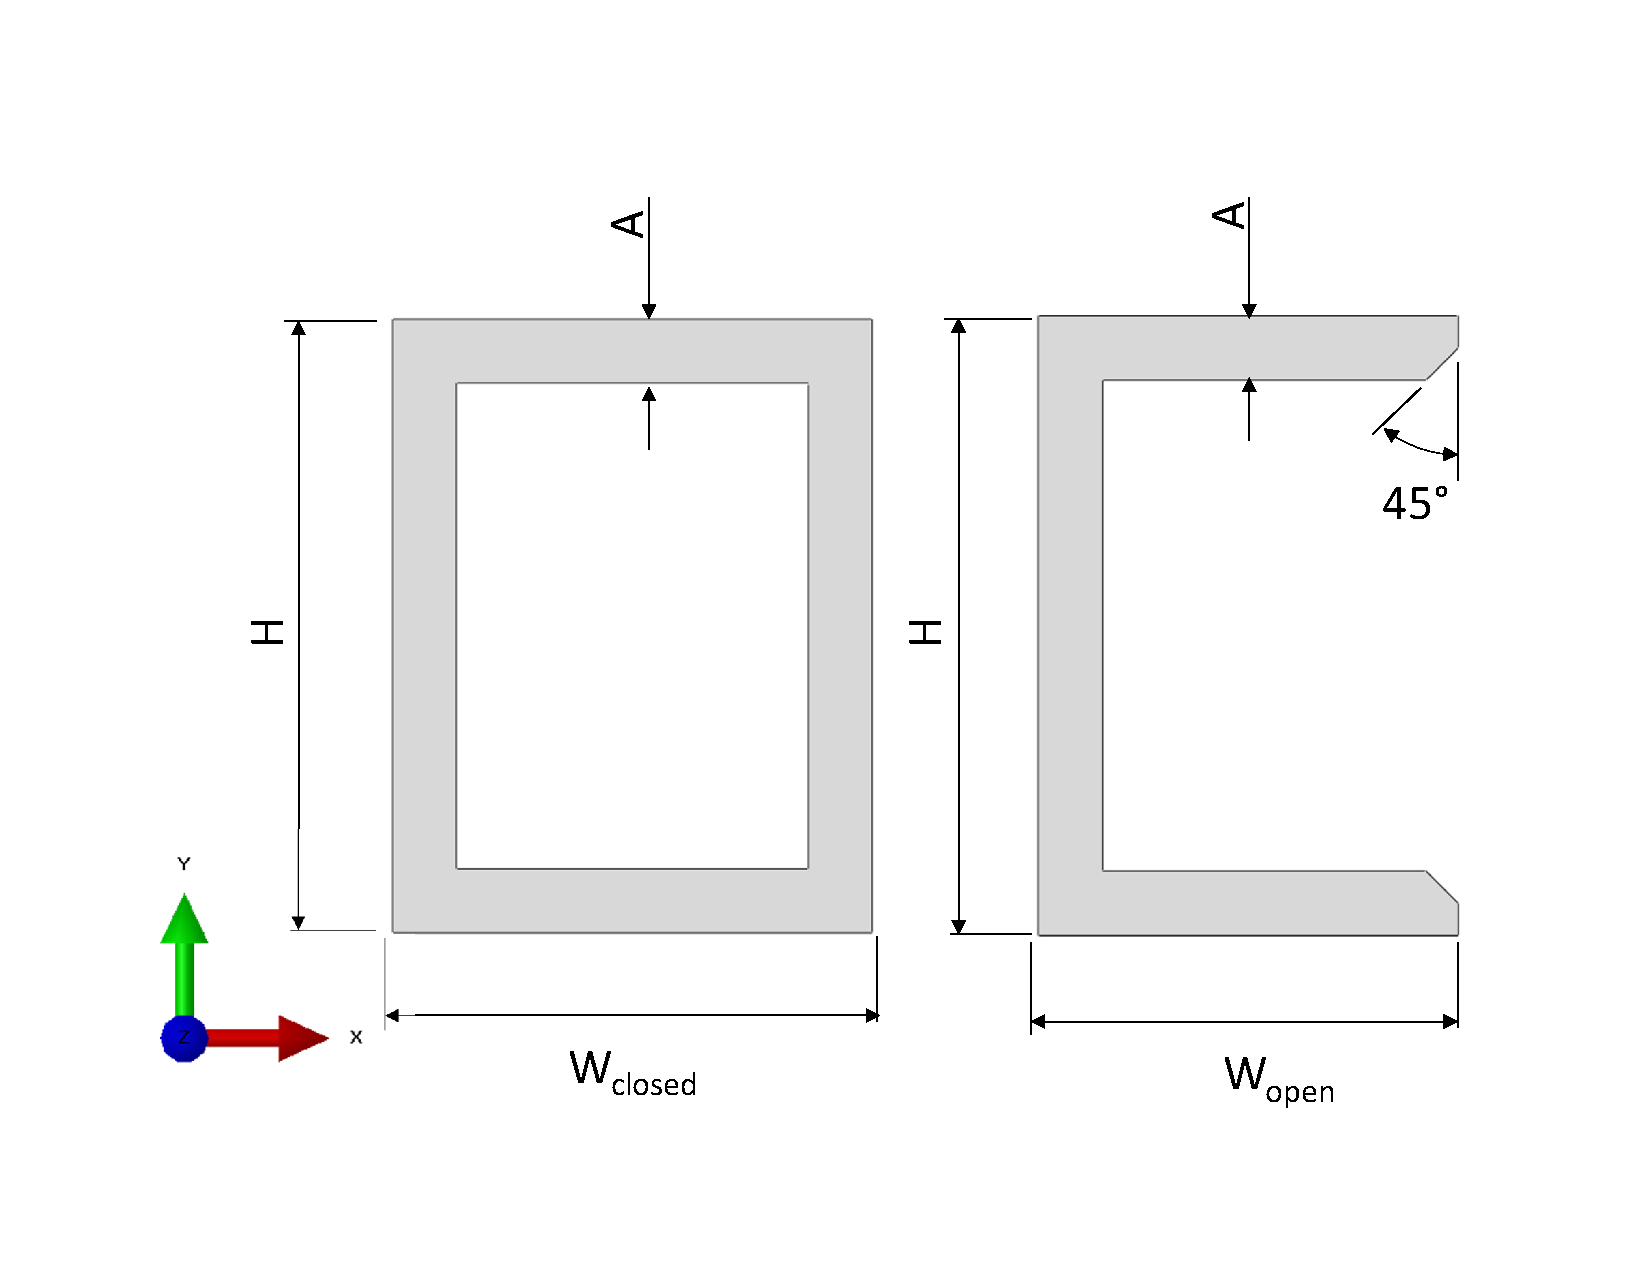
\includegraphics[width=0.8 \textwidth]{model/rib-internalParameters}
  \caption[Internal parameters of the two different ribs parts]{Internal parameters of the two different ribs parts.}\label{fig:rib-internalParameters}
\end{figure}

Therefore, the only tailorable parameters for the ribs configurations are the thickness $t_{\mathrm{rib}}$ and the frame width $A_{\mathrm{rib}}$. The nominal value and units of these two parameters together with the nominal value and units of the remaining dependent parameters can be read in Table \ref{tab:parameters_rib}. The Young's modulus was increase one order of magnitude in comparison of that of the wing-box in order to ensure no out-of-plane deformation of the rib.

\begin{table}[!htpb]
\centering
\begin{tabular}{|l|lll|}
\hline
\textbf{Parameter} & \multicolumn{1}{l|}{\textbf{Symbol}} & \multicolumn{1}{l|}{\textbf{Units}} & \textbf{Nominal value} \\ \hline \hline
{\textbf{Dimensions}} &  &  &  \\ \hline
Rib height & \multicolumn{1}{l|}{$H_{\mathrm{rib}}$} & \multicolumn{1}{l|}{mm} & 383.27 \\ \hline
Closed rib width & \multicolumn{1}{l|}{$W_{\mathrm{rib,close}}$} & \multicolumn{1}{l|}{mm} & 300 \\ \hline
Frame width & \multicolumn{1}{l|}{$A_{\mathrm{rib}}$} & \multicolumn{1}{l|}{mm} & 30 \\ \hline
Rib thickness & \multicolumn{1}{l|}{$t_{\mathrm{rib}}$} & \multicolumn{1}{l|}{mm} & 2 \\ \hline \hline
{\textbf{Material (Aluminum, 10xE)}} &  &  &  \\ \hline
Young's modulus & \multicolumn{1}{l|}{$E_{\mathrm{box}}$} & \multicolumn{1}{l|}{N/mm$^2$} & 690000 \\ \hline
Poisson's ratio & \multicolumn{1}{l|}{$\nu_{\mathrm{box}}$} & \multicolumn{1}{l|}{} & 0.3269 \\ \hline
\end{tabular}
\caption[Parameters used for the ribs model]{Parameters used for the ribs model. The Young's modulus was increase one order of magnitude in comparison of that of the wing-box in order to ensure no out-of-plane deformation of the rib. The value of the rib width $W_{\mathrm{rib,close}}$ and the height $H_{\mathrm{rib}}$ will be equal to the wing-box width $W_{\mathrm{box}}$ and to the chiral lattice structure height, respectively.}
\label{tab:parameters_rib}
\end{table}

\clearpage
\subsection{Model mesh} \label{subsec:mesh_computationalModel}

In the present section, the mesh used in the model will be presented. The mesh was unstructured and it was auto-generated by Abaqus CAE for the whole assembly. The elements were a combination of quadratic and tetrahedral with 4 and 3 nodes, respectively. Different mesh elements size were assigned to different parts of the model depending of the stress complexity expected. 

In Figure \ref{fig:mesh}, it is possible to distinguish two regions that were assigned with different mesh size: the lattice structure and near region of the wing-box skin was assigned with a fine mesh size while the remaining model was assigned with a course mesh, typically one order of magnitude greater.

\begin{figure}[!htpb]
  \centering
  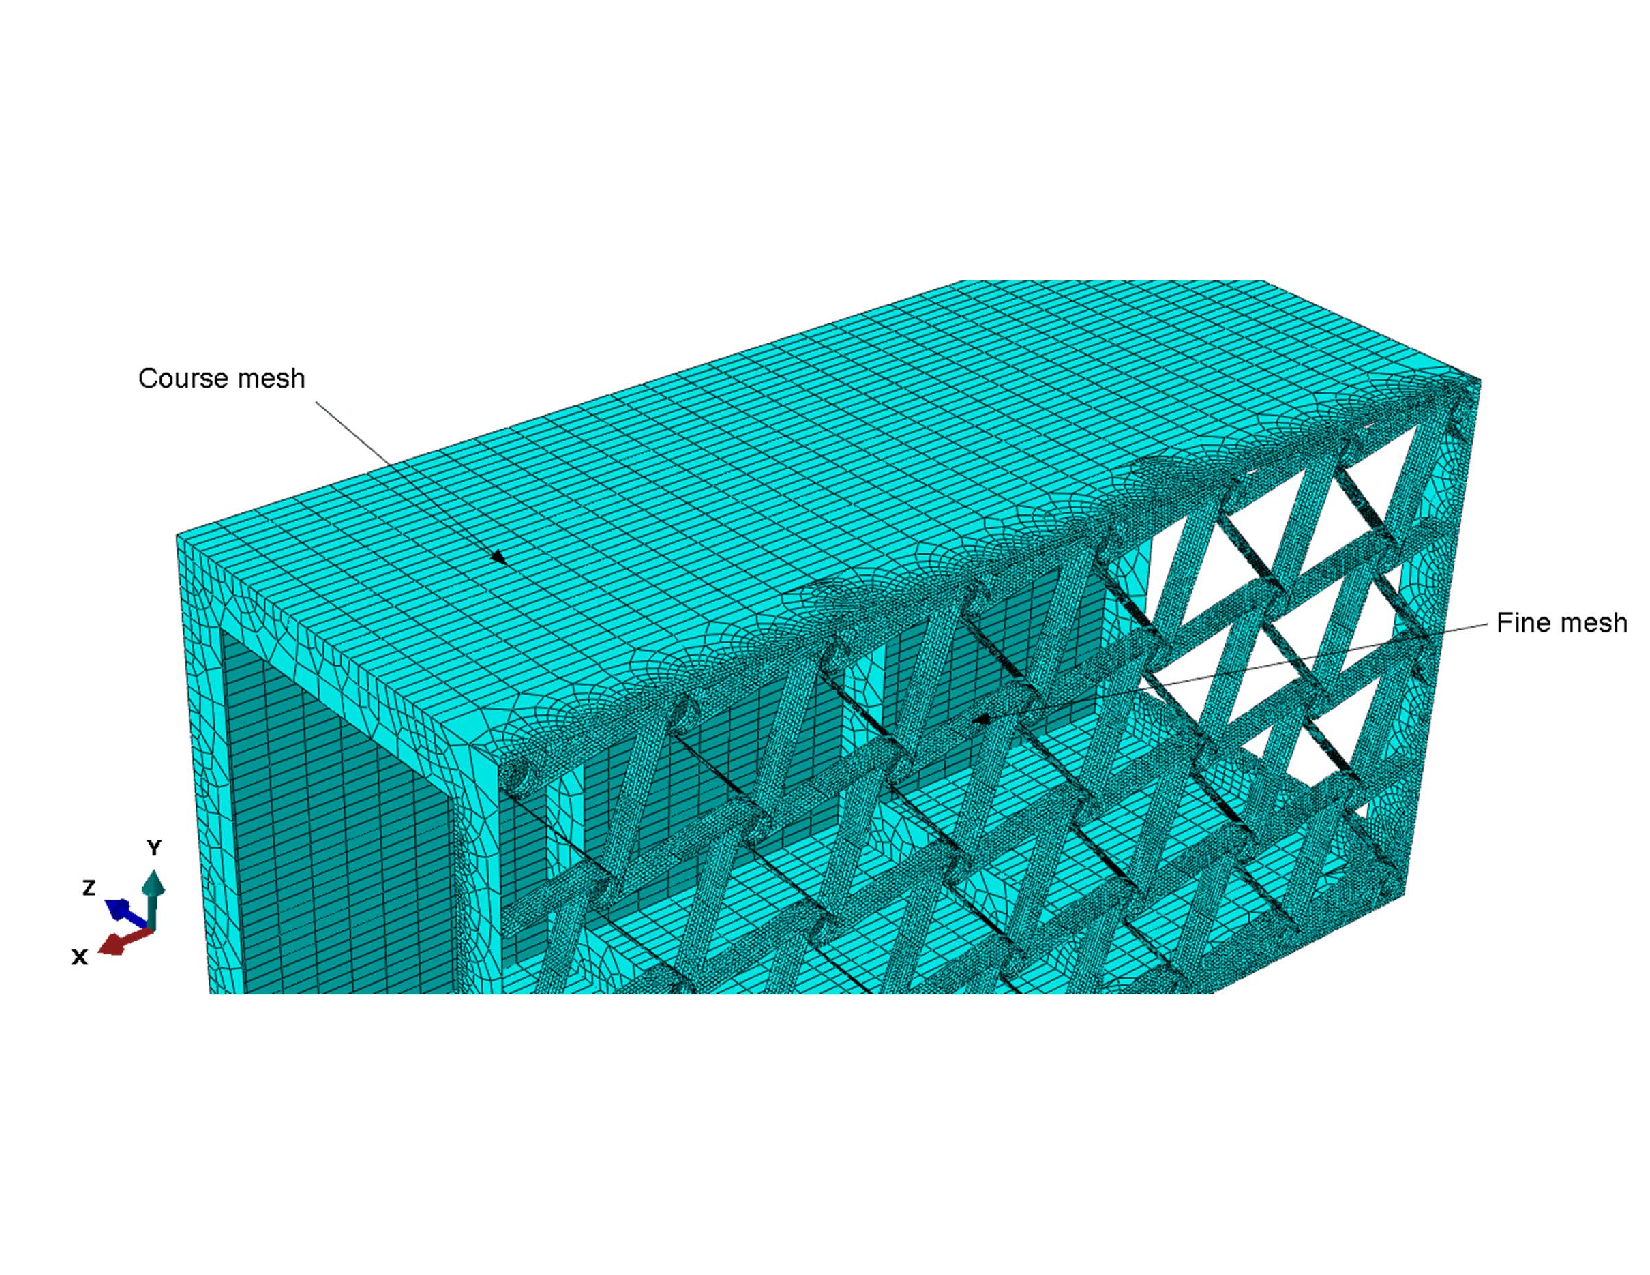
\includegraphics[width=0.8 \textwidth]{model/mesh}
  \caption[Internal parameters of the two different ribs parts]{Internal parameters of the two different ribs parts. Different mesh elements size were assigned to different parts of the model. The lattice structure was assigned with a fine mesh element size while the wing-box was assigned with a course mesh element size.}\label{fig:mesh}
\end{figure}

\clearpage
\subsection{Attachment points modeling} \label{subsec:connections_computationalModel}

%General thoughts:
% - Necessity of applying condition node to node
%
%Equation contrainsts issues:
% - Slow down simulations
%
%Coupling constrainsts:
%
%
In the present subsection, the FEM modeling of the connection between the lattice nodes and the wing box is presented. This is an unavoidable transition from the lattice structure of nodes and ligaments to the skin of the wing box. Loads are transmitted to the lattice through this attachment points that is why its design results crucial.

There will be three different configurations that were studied:

\begin{description}
  \item[Blocked translation and rotation] The lattice nodes have all its degrees of freedom restrained
  \item[Blocked translation and free rotation] The lattice nodes are free to rotate around its own axis but the translation the direction parallel to the skin is restrained. An sketch showing this connection can be viewed in Figure \ref{fig:connectionModeling1}. This configuration was the one chosen for the demonstrator built in the Figure \ref{fig:connectionLatticeNodesToSkin-tobeimproved}.
  \item[Free translation and rotation] Now the lattice nodes is allowed to translate parallel to the skin. This configuration is schematically represented in Figure \ref{fig:connectionModeling2}.
\end{description}

\begin{figure}[!htpb]
  \centering
  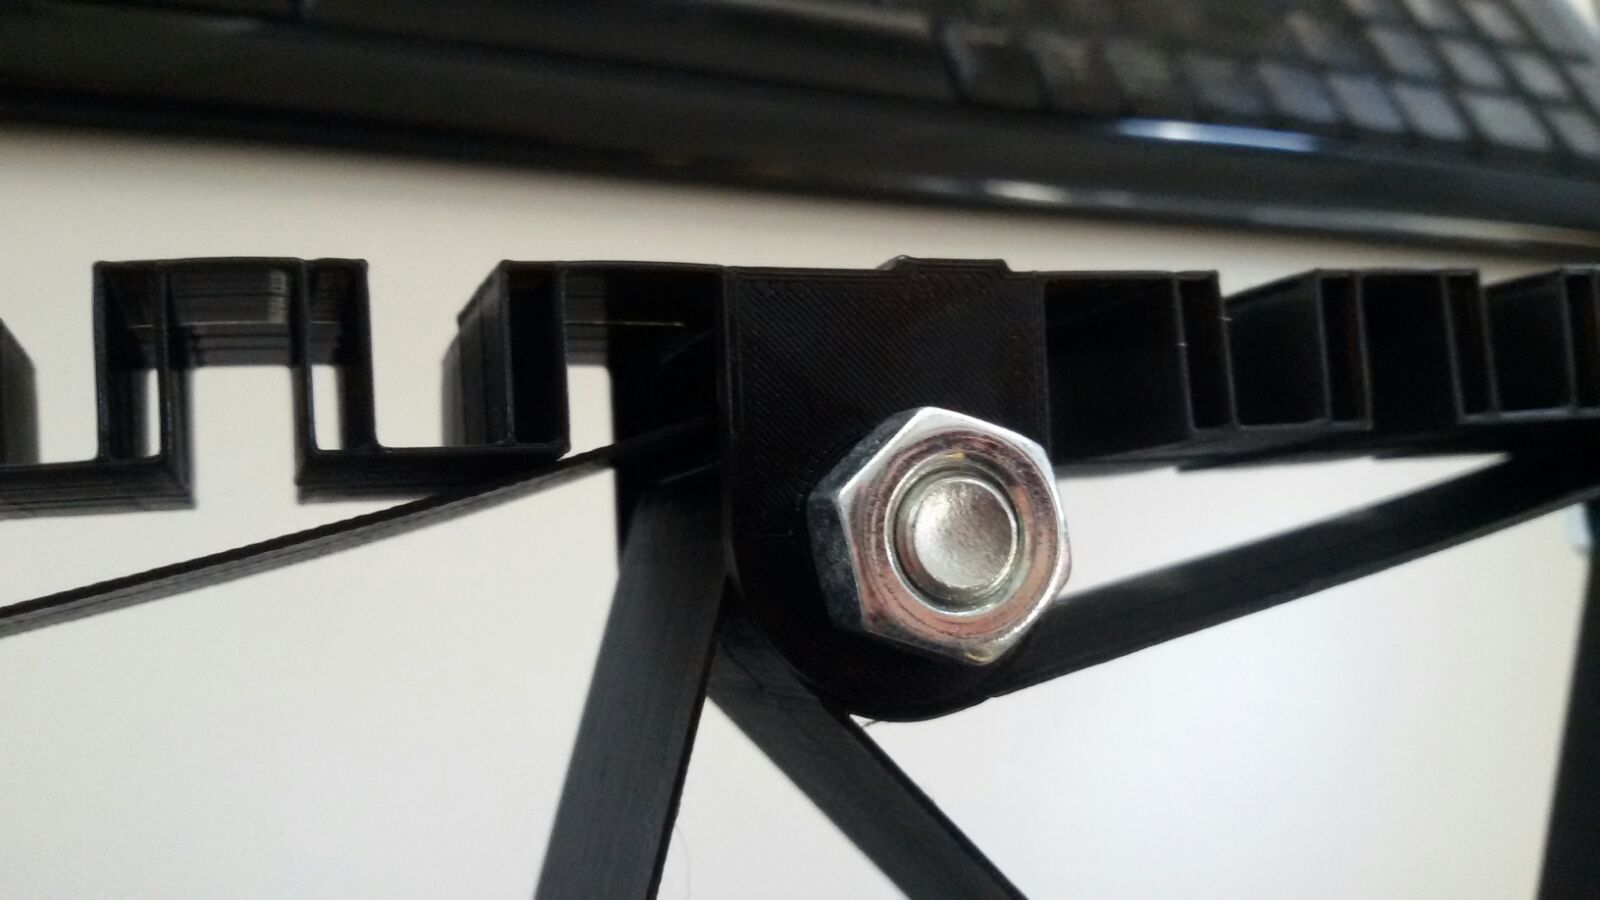
\includegraphics[width=0.8 \textwidth]{model/connectionLatticeNodesToSkin-tobeimproved}
  \caption[Detail of the connection between the lattice nodes and the skin]{Detail of the connection between the lattice nodes and the skin. The picture shows the type of connection chosen for the manufactured demonstrator of the lattice. The lattice nodes is allowed to rotate around its own axis but cannot translate parallel to the skin. \cite{Vincenz2017}}\label{fig:connectionLatticeNodesToSkin-tobeimproved}
\end{figure}

\begin{figure}[!htpb]
  \centering
  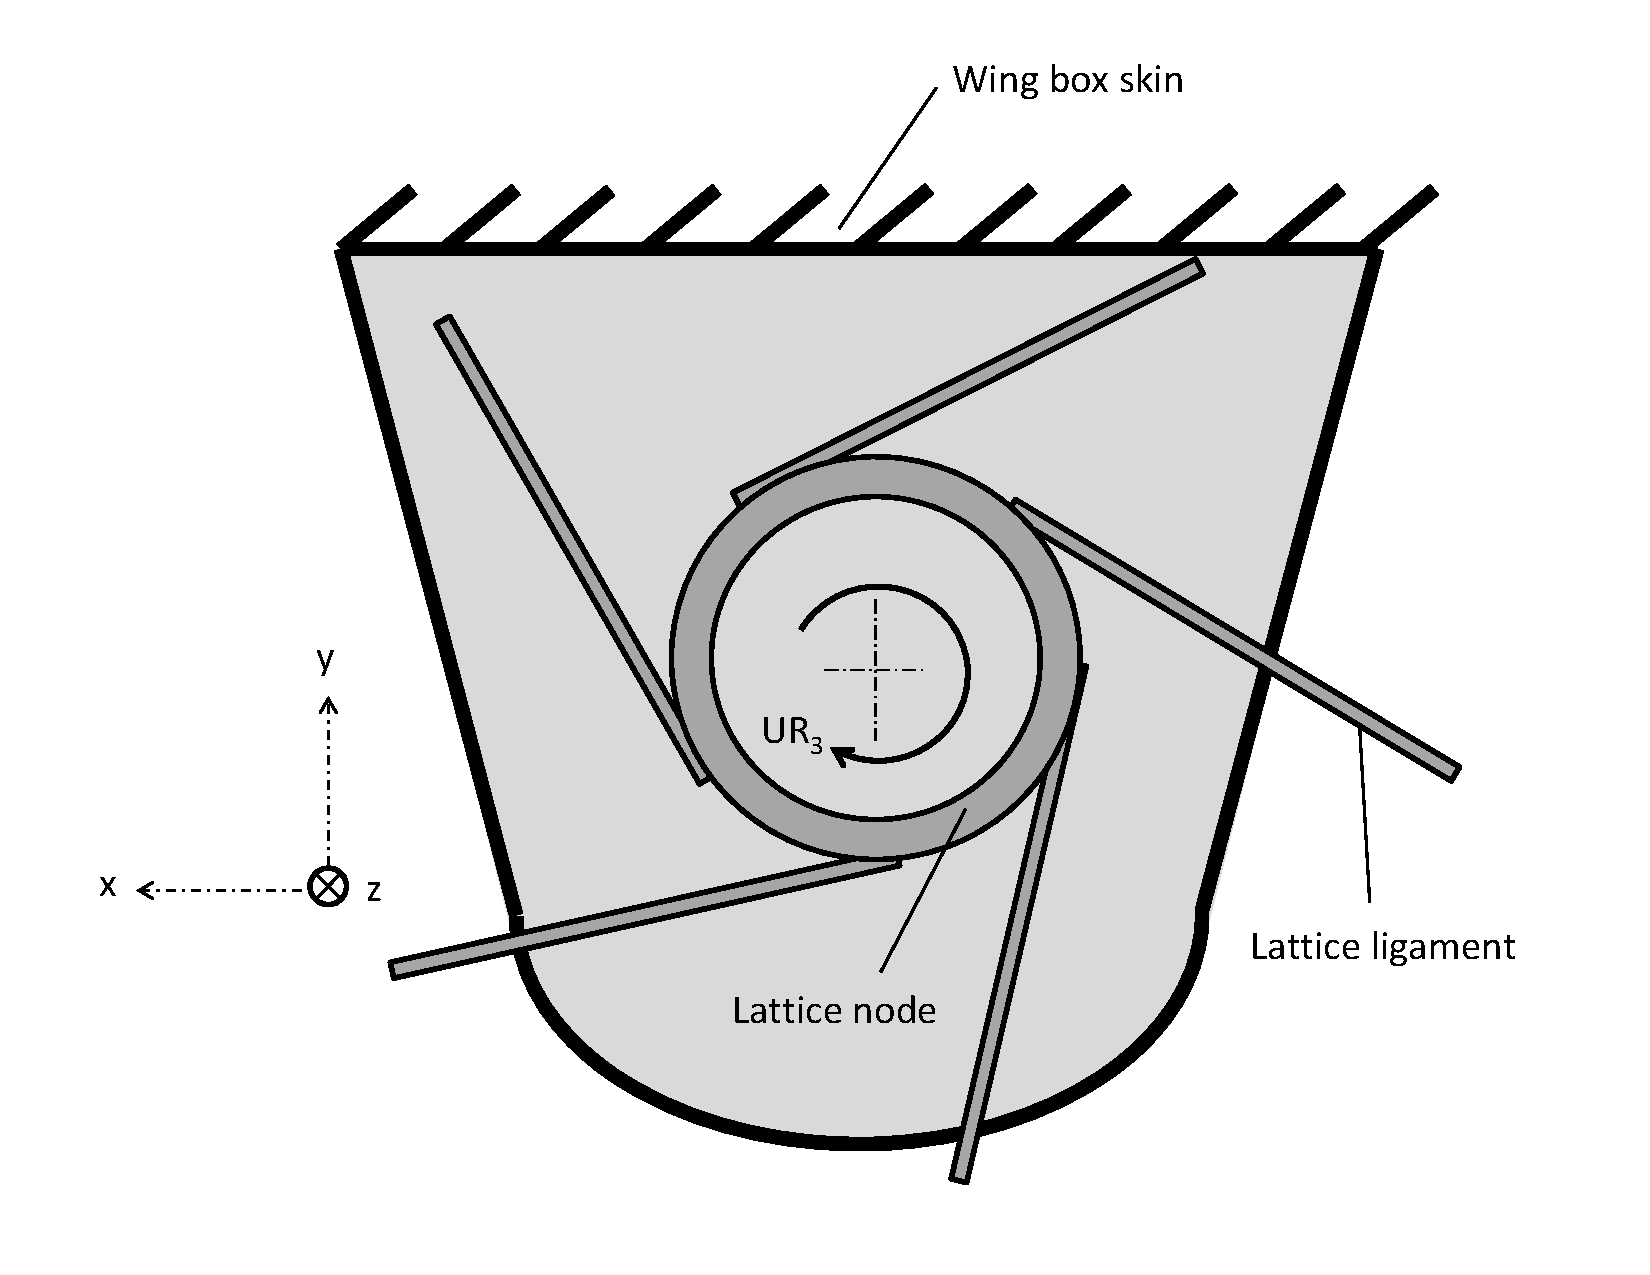
\includegraphics[width=0.8 \textwidth]{model/connectionModeling1}
  \caption[Blocked translation and free rotation connection between the lattice nodes and the skin]{Blocked translation and free rotation connection between the lattice nodes and the skin. In this case, the only degree of freedom of the lattice node that it is not restrained the rotation around its own axis, that is the rotation $UR_3$ around the direction $z$.}\label{fig:connectionModeling1}
\end{figure}

\begin{figure}[!htpb]
  \centering
  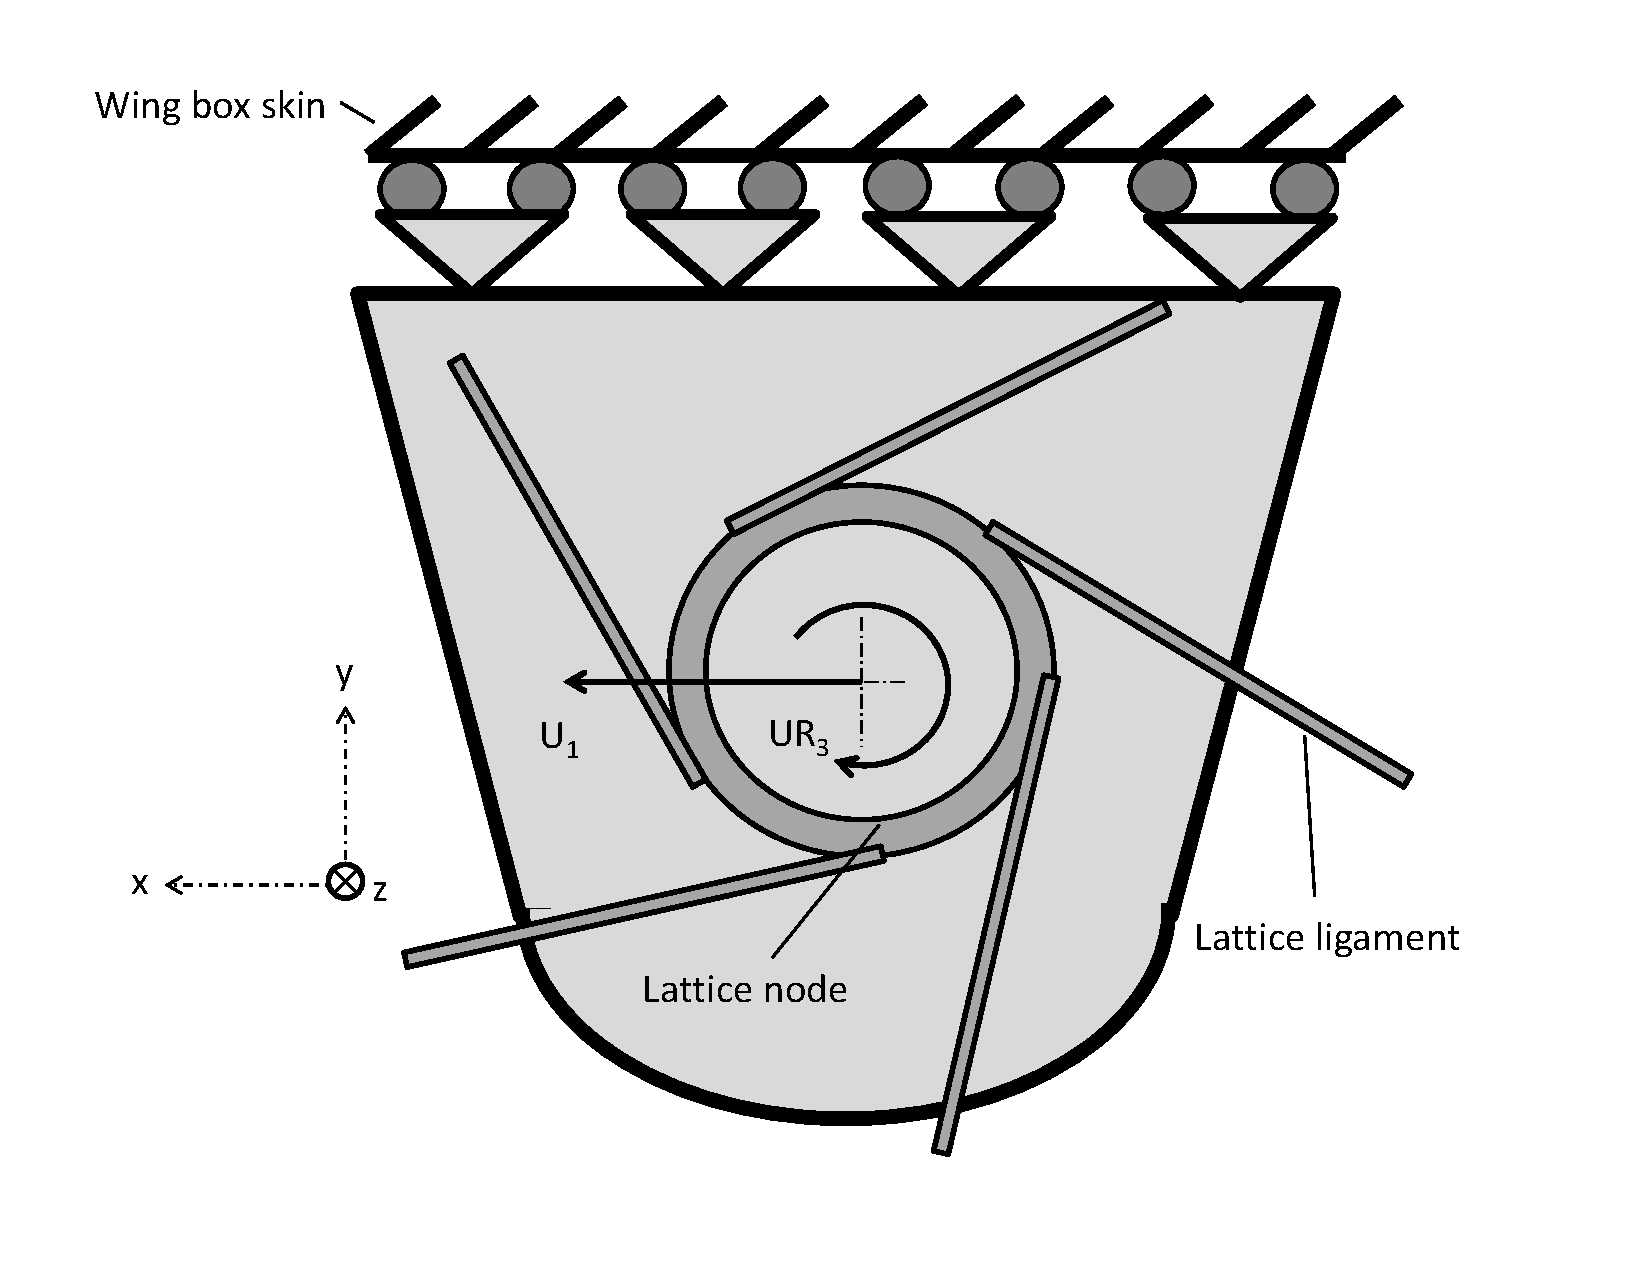
\includegraphics[width=0.8 \textwidth]{model/connectionModeling2}
  \caption[Free translation and rotation connection between the lattice nodes and the skin]{Free translation and rotation connection between the lattice nodes and the skin. For this case, the unrestrained degrees of freedom of the lattice nodes are the rotation the rotation $UR_3$ around its own axis, i.e.: the direction $z$; and the displacement $U_1$ parallel to the wing-box wall, i.e.: along the direction $x$.}\label{fig:connectionModeling2}
\end{figure}

In the FEM model, the three connections where modeled using different approaches. Since the lattice of chiral elements and the skin of the wing box were not physical connected by any element, it was necessary to use of the interaction modules provided by Abaqus CAE. There a different options available to constrain the degrees of freedom of a particular set of mesh nodes to another set of mesh nodes. Some of these modules were already explored in Subsection \ref{subsec:parametrization_Model} when investigating how to model the lattice nodes rigid body behavior.

\subsubsection{Coupling through tyre part}

This approach consisted in using the tyre part that was described in Subsection \ref{subsec:parametrization_Model}. In each of the lattice nodes located at the border of the lattice structure, a tyre part was created and embed into the lattice node, as it was shown in Figure \ref{fig:tyre-connection}. Then, a coupling constraint is establish between a mesh node in the middle of the tyre and a mesh node located on the wing-box skin just above the tyre, as shown in Figure \ref{fig:connection-tyre}.

\begin{figure}[!htpb]
  \centering
  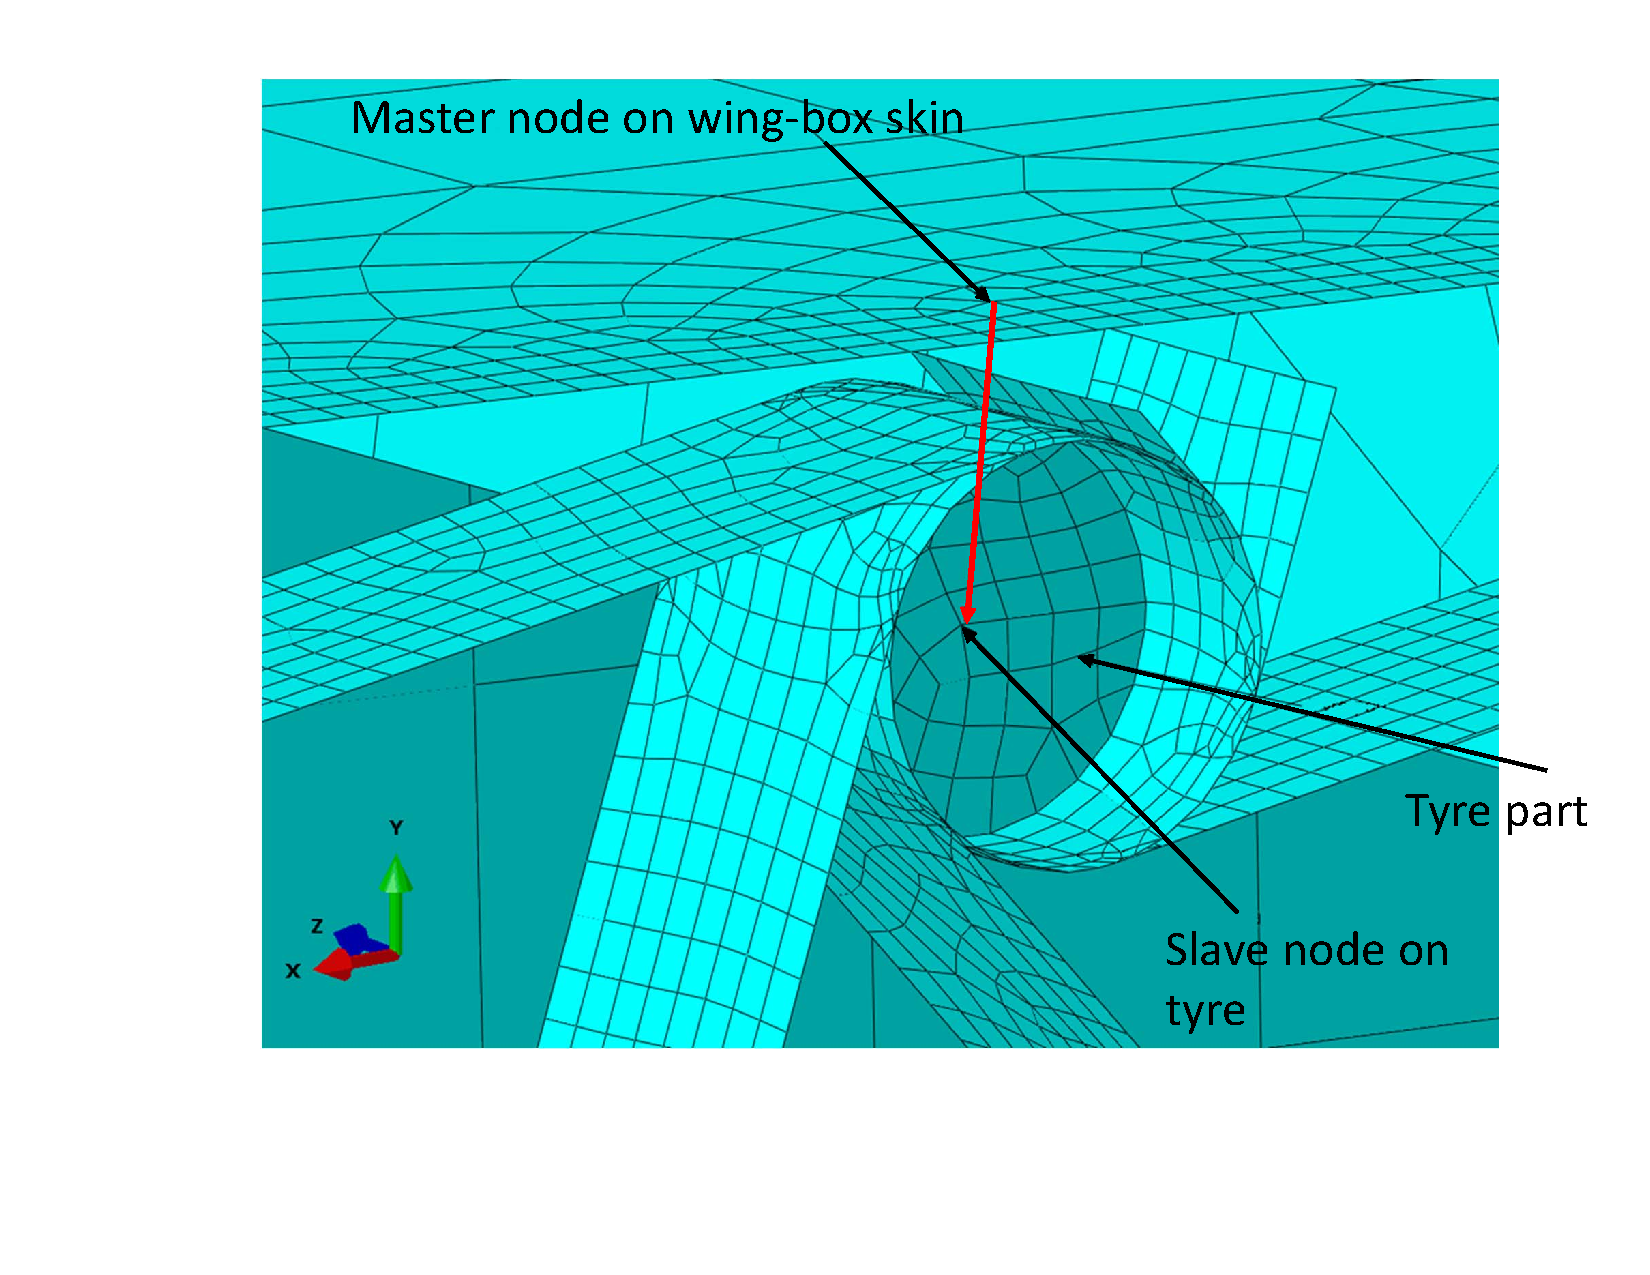
\includegraphics[width=0.8 \textwidth]{model/connection-tyre}
  \caption[Coupling condition between the lattice node and the wing-box skin through tyre]{Coupling condition between the lattice node and the wing-box skin through tyre. The coupling condition is establish between a mesh node located in the wing-box skin that acts as a master node and a mesh node in the middle of the tyre that becomes the coupling node.}\label{fig:connection-tyre}
\end{figure}

Depending on the type of connection considered, there will be different degrees of freedom the ones that are coupled. For the most restrictive case, in which the connection between the lattice structure and the wing-box is rigid, not allowing any displacement, the six degrees of freedom will be coupled between the mesh nodes mentioned on the previous paragraph.

For the other connection types, rotation of the lattice node is allowed around its own axis. This allowance is implemented by not constraining the rotation $UR_3$ around the $z$ direction in the coupling constraint definition. Finally, the last connection type explained at the beginning of the present subsection allowed the displacement of the lattice node parallel to the wing-box skin. For this case, the translation $U_1$ along the $x$ direction is be left uncoupled.

The rigid body motion imposed to the mesh node located at the center of the tyre is translated to the mesh nodes located in the faces of the lattice node because they are physically connected.

\subsubsection{Coupling through local cylindrical reference system}

In this case, the function provided by the tyre is substituted by an additional coupling condition. This links a reference point located at the centre of the lattice node to the mesh nodes located . As rotation is allowed in the nodes located in t POR AQUÍ ME QUEDÉ ESCRIBIENDO

\begin{figure}[!htpb]
  \centering
  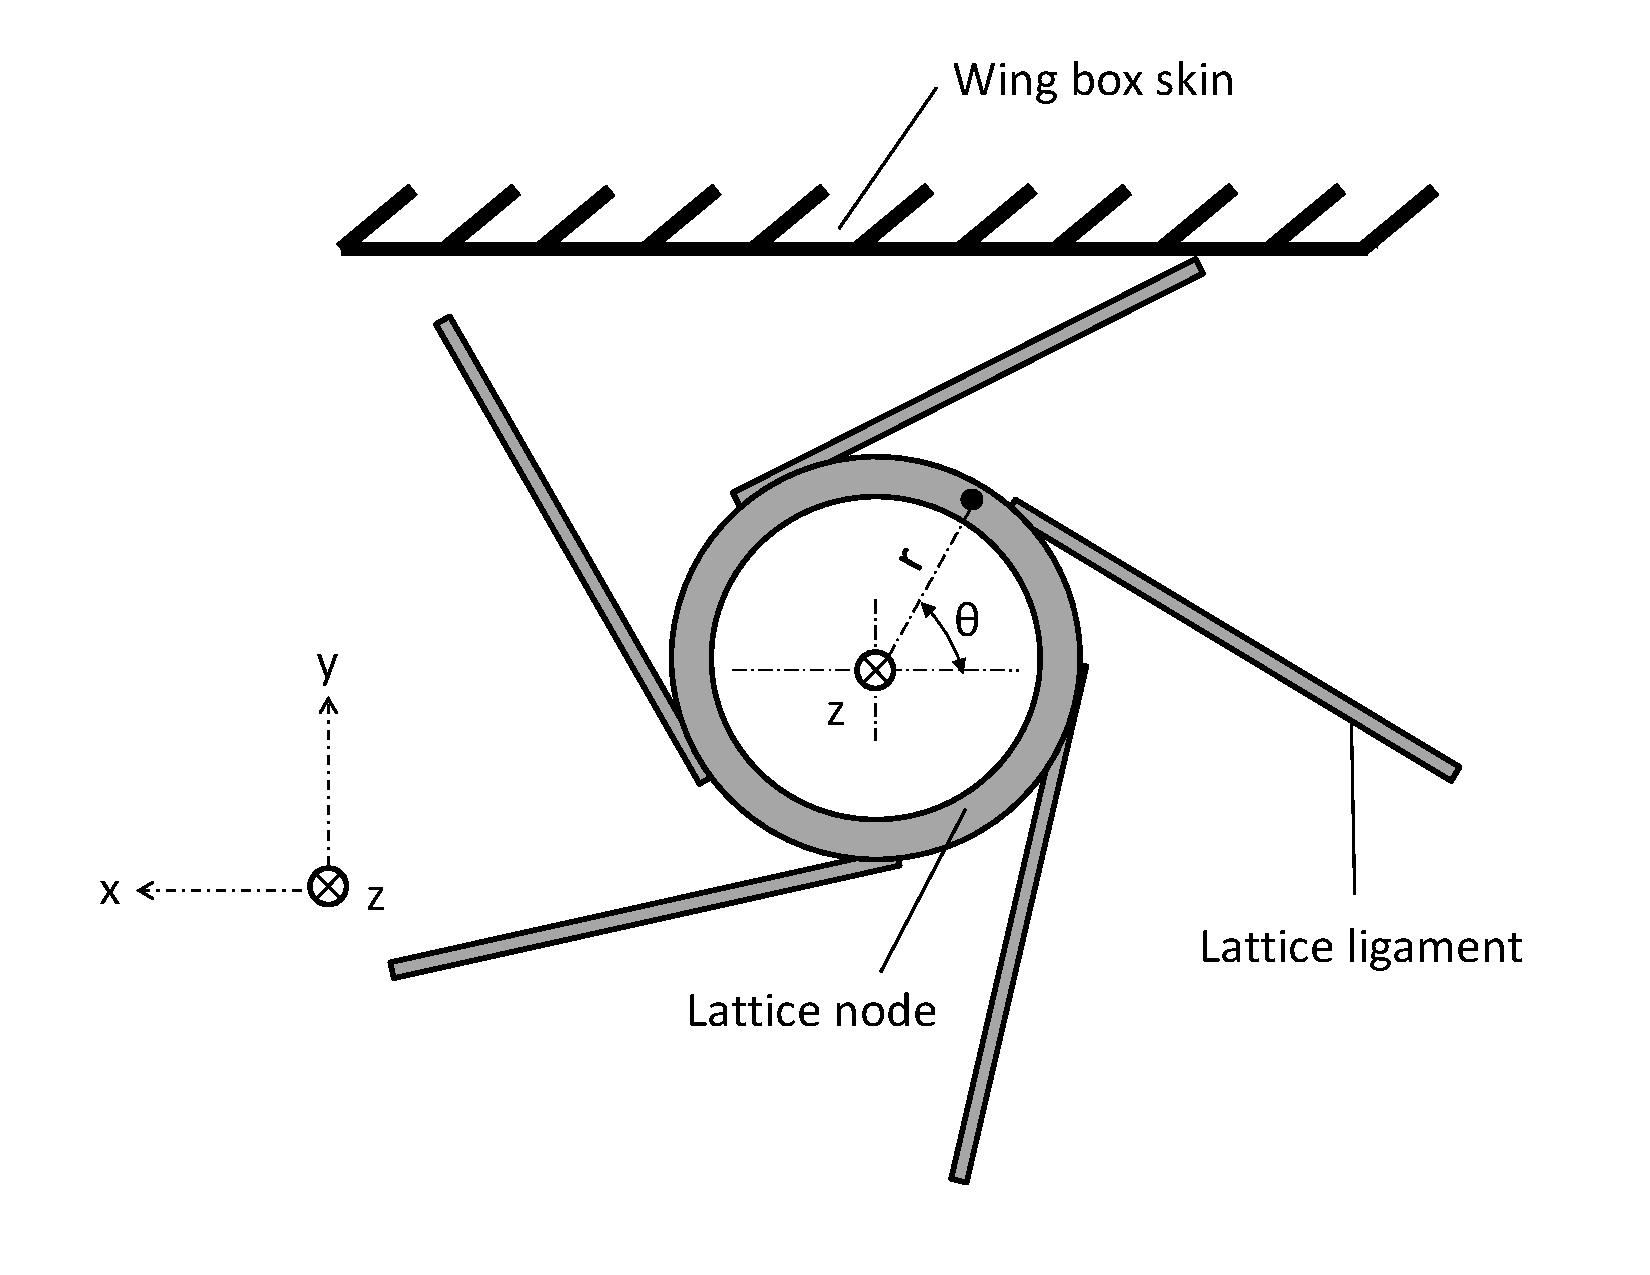
\includegraphics[width=0.8 \textwidth]{model/connection-SYS1}
  \caption[Local reference system at the lattice nodes]{Local reference system at the lattice nodes. }\label{fig:connection-sys1}
\end{figure}

\begin{figure}[!htpb]
  \centering
  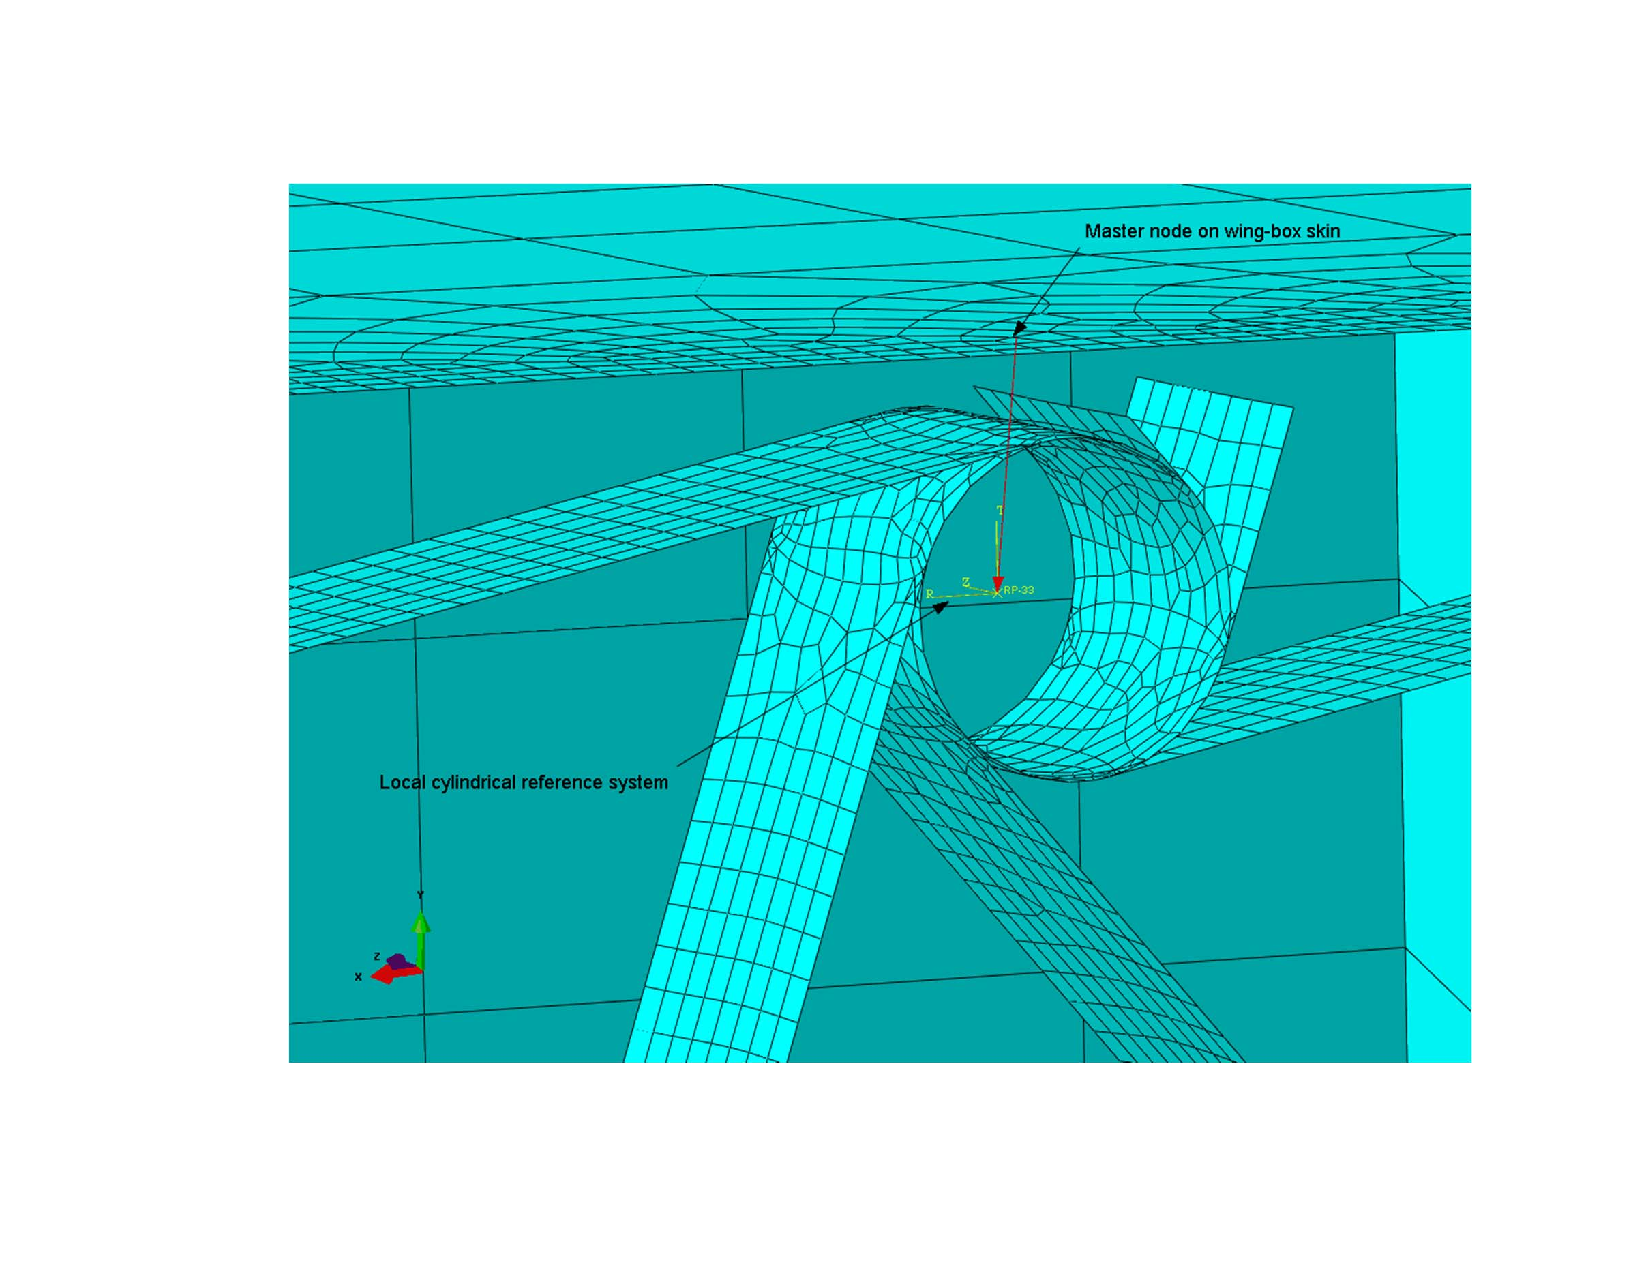
\includegraphics[width=0.8 \textwidth]{model/connection-SYS2}
  \caption[Coupling condition between the lattice node and the wing-box skin through local reference system]{Coupling condition between the lattice node and the wing-box skin through local reference system. }\label{fig:connection-sys2}
\end{figure}

\clearpage
\subsection{Parametric study method} \label{subsec:parametricStudy_computationalModel} 